%% File encoding: UTF-8
%% äöüÄÖÜß  <-- keine deutschen Umlaute hier? UTF-faehigen Editor verwenden!

\documentclass[bachelor,german]{hgbthesis}
% Zulässige Class Options: 
%   Typ der Arbeit: diplom, master (default), bachelor, praktikum 
%   Hauptsprache: german (default), english
%%------------------------------------------------------------

\RequirePackage[utf8]{inputenc}		% remove when using lualatex oder xelatex!

\graphicspath{{images/}}    % name of directory containing the images
\logofile{logo}							% name of logo-PDF in images/ (or use \logofile{} for no logo)
\bibliography{literatur}  	% name of the BibTeX (.bib) file

\usepackage{listings}
\usepackage{graphicx}
\usepackage{tikz}
\usepackage{pgfplots}
\usepackage{subfig}
\usetikzlibrary{
  arrows.meta, % for Straight Barb arrow tip
  fit, % to fit the group box around the central neurons
  positioning, % for relative positioning of the neurons
}

\tikzset{
  neuron/.style={ % style for each neuron
    circle,draw,thick, % drawn as a thick circle
    inner sep=5pt, % no built-in padding between the text and the circle shape
    minimum size=1.5em, % make each neuron the same size regardless of the text inside
    node distance=1ex and 3em, % spacing between neurons (y and x)
  },
  group/.style={ % style for the groups of neurons
    rectangle,%,draw,thick, % drawn as a thick rectangle
    inner sep=0pt, % no padding between the node contents and the rectangle shape
  },
  io/.style={ % style for the inputs/outputs
    neuron, % inherit the neuron style
    fill=gray!15, % add a fill color
  },
  conn/.style={ % style for the connections
    -{Straight Barb[angle=60:2pt 3]}, % simple barbed arrow tip
    thick, % draw in a thick weight to match other drawing elements
  },
}

%%%----------------------------------------------------------
\begin{document}
%%%----------------------------------------------------------

% Einträge für ALLE Arbeiten: --------------------------------
\title{Machine Learning und tiefe neuronale Netze mit TensorFlow}
\author{David Baumgartner}
\studiengang{Software Engineering}
\studienort{Hagenberg}
\abgabedatum{2017}{01}{14}	% {YYYY}{MM}{DD}

%%% zusätzlich für eine Bachelorarbeit: ---------------------
\nummer{XXXXXXXXXX-A}   % XX...X = Stud-ID, z.B. 0310238045-A  
                        % (A = 1. Bachelorarbeit)
\semester{Wintersemester 2016/17} 
\gegenstand{………………}%Einführung in die Tiefere Problematik 1} 
\betreuer{Stephan Dreiseitl, FH-Prof. PD DI Dr.} % oder \betreuerin{..}

%%% zusätzlich für einen Praktikumsbericht: -----------------
%\nummer{XXXXXXXXXX-B}   % XX...X = Stud-ID, z.B. 0310238045-B  
                        % (B = 2. Bachelorarbeit)
%\betreuer{Mag.~Pjotr I.~Czar\\Creative Director}  % \betreuerin{..}
%\firma{%
%   Oligarchic Media International GmbH\\
%   Online Division\\
%   1020 Wien, Hubertusgasse 3a
%}
%\firmenTel{1-234-5678-100}
%\firmenUrl{www.mogul.at}

%\strictlicense  % erzeugt restriktive Lizenzformel

%%%----------------------------------------------------------
\frontmatter
\maketitle
\tableofcontents
%%%----------------------------------------------------------

\chapter{Vorwort} 	% engl. Preface


Dies ist \textbf{Version \hgbthesisDate} der \latex-Dokumentenvorlage für 
verschiedene Abschlussarbeiten an der Fakultät für Informatik, Kommunikation
und Medien der FH Oberösterreich in Hagenberg, die mittlerweile auch 
an anderen Hochschulen im In- und Ausland gerne verwendet wird.

Das Dokument entstand ursprünglich auf Anfragen von Studierenden,
nachdem im Studienjahr 2000/01 erstmals ein offizieller
\latex-Grundkurs im Studiengang Medientechnik und -design an der
FH Hagenberg angeboten wurde. Eigentlich war die Idee, die bereits
bestehende \emph{Word}-Vorlage für Diplomarbeiten "`einfach"' in
\latex\ zu übersetzen und dazu eventuell einige spezielle
Ergänzungen einzubauen. Das erwies sich rasch als wenig
zielführend, da \latex, \va was den Umgang mit Literatur und
Grafiken anbelangt, doch eine wesentlich andere Arbeitsweise
verlangt. Das Ergebnis ist -- von Grund auf neu geschrieben und
wesentlich umfangreicher als das vorherige Dokument --
letztendlich eine Anleitung für das Schreiben mit \latex, ergänzt
mit einigen speziellen (mittlerweile entfernten) Hinweisen für \emph{Word}-Benutzer.
Technische Details zur aktuellen Version finden sich in Anhang \ref{ch:TechnischeInfos}.

Während dieses Dokument anfangs ausschließlich für die Erstellung
von Diplomarbeiten gedacht war, sind nunmehr auch  
\emph{Masterarbeiten}, \emph{Bachelor\-arbeiten} und \emph{Praktikumsberichte} 
abgedeckt, wobei die Unterschiede bewusst gering gehalten wurden.

Bei der Zusammenstellung dieser Vorlage wurde versucht, mit der
Basisfunktionalität von \latex das Auslangen zu finden und -- soweit möglich --
auf zusätzliche Pakete zu verzichten. Das ist nur zum Teil gelungen;
tat\-säch\-lich ist eine Reihe von ergänzenden "`Paketen"' notwendig, wobei jedoch
nur auf gängige Erweiterungen zurückgegriffen wurde.
Selbstverständlich gibt es darüber hinaus eine Vielzahl weiterer Pakete,
die für weitere Verbesserungen und Finessen nützlich sein können. Damit kann
sich aber jeder selbst beschäftigen, sobald das notwendige Selbstvertrauen und
genügend Zeit zum Experimentieren vorhanden sind.
Eine Vielzahl von Details und Tricks sind zwar in diesem Dokument nicht explizit
angeführt, können aber im zugehörigen Quelltext jederzeit ausgeforscht
werden.

Zahlreiche KollegInnen haben durch sorgfältiges Korrekturlesen und
konstruktive Verbesserungsvorschläge wertvolle Unterstützung
geliefert. Speziell bedanken möchte ich mich bei Heinz Dobler für
die konsequente Verbesserung meines "`Computer Slangs"', bei
Elisabeth Mitterbauer für das bewährte orthographische Auge und
bei Wolfgang Hochleitner für die Tests unter Mac~OS.

Die Verwendung dieser Vorlage ist jedermann freigestellt und an
keinerlei Erwähnung gebunden. Allerdings -- wer sie als Grundlage
seiner eigenen Arbeit verwenden möchte, sollte nicht einfach
("`ung'schaut"') darauf los werken, sondern zumindest die
wichtigsten Teile des Dokuments \emph{lesen} und nach Möglichkeit
auch beherzigen. Die Erfahrung zeigt, dass dies die Qualität der
Ergebnisse deutlich zu steigern vermag.

Der Quelltext zu diesem Dokument sowie das zugehörige
\latex-Paket sind in der jeweils aktuellen Version online
verfügbar unter
%
\begin{itemize}
\item[]\url{https://sourceforge.net/projects/hgbthesis/}.
\end{itemize}
%
Trotz großer Mühe enthält dieses Dokument zweifellos Fehler und Unzulänglichkeiten
-- Kommentare, Verbesserungsvorschläge und passende Ergänzungen
sind daher stets willkommen, am einfachsten per E-Mail direkt an mich:
\begin{itemize}
\item[]%

Dr.\ Wilhelm Burger, Department für Digitale Medien,\newline
Fachhochschule Oberösterreich, Campus Hagenberg (Österreich)\newline
\nolinkurl{wilhelm.burger@fh-hagenberg.at}
\end{itemize}

\noindent
Übrigens, hier im Vorwort (das bei Diplom- und Masterarbeiten üblich, bei Bachelorarbeiten 
aber entbehrlich ist) kann kurz auf die Entstehung des Dokuments eingegangen werden.
Hier ist auch der Platz für allfällige Danksagungen (\zB an den Betreuer, 
den Begutachter, die Familie, den Hund, \ldots), Widmungen und philosophische 
Anmerkungen. Das sollte allerdings auch nicht übertrieben werden und sich auf 
einen Umfang von maximal zwei Seiten beschränken.




		% ggfs. weglassen

\chapter{Kurzfassung}

Maschinelles lernen und tiefe neuronale Netze werden unter anderem in 
unserem Jahrzehnt sehr häufig eingesetzt um technische Problemstellungen 
zu lösen, für des eine in vernünftiger Zeit keine Brauchbaren 
iterative Algorithmen gibt. Zusätzlich werden maschinell 
lernende System immer häufiger in unserem allgemeinen Alttag 
eingesetzt um uns zu unterstützen und um von den Benützern zu lernen.
Ein neuronales Netzwerk kann aber nicht einfach erstellt werden
und im nächsten Schritt in der Praxis eingesetzt werden. Dies würde 
zu erheblichen Problemen führen. Diese Netzwerke müssen trainiert werden
sowie getestet. 


Im Rahmen dieser Bachelorarbeit werden die wichtigsten theoretischen Konzepte zu 
maschinellem lernen und tiefe neuronale Netze theoretisch zu vergleichen und empirisch zu überprüfen. 
Dazu wird das TensorFlow-Bibliothek als Beispiel verwendet und analysiert. Aus dieser Bibliothek werden 
die benötigten Teile heraus genommen und in einem Python-Script zusammen gefügt um in Bildern mit Gesichtern 
gewisse Züge zu erkennen und zu Klassifizieren. Durch die Analysephasen werden theoretische und berechnete Annahmen 
untermauert oder in Frage gestellt. Folgende Schlussfolgerungen gehen jedoch nach Auswertung 
der Ergebnisse über die theoretischen Annahmen hinaus: Ist das TensorFlow-System 
in der Lage, Muster aus unterschiedlichen Datentypen, wie zum Beispiel Bilder, 
Videos oder Videostreams, zu erkennen und von diesen selbst zu lernen?

Die Bachelorarbeit ist sowohl für Studierende im Studium Software Engineering sowie 
Informatik als auch für Lehrende in diesen Bereichen interessant.




%An dieser Stelle steht eine Zusammenfassung der Arbeit, Umfang
%max.\ 1 Seite. Im Unterschied zu anderen Kapiteln ist die
%Kurzfassung (und das Abstract) üblicherweise nicht in Abschnitte
%und Unterabschnitte gegliedert. 
%Auch Fußnoten sind hier falsch am Platz.
%
%Kurzfassungen werden übrigens häufig -- zusammen mit Autor und Titel
%der Arbeit -- %
%in Literaturdatenbanken aufgenommen. Es ist daher darauf zu
%achten, dass die Information in der Kurzfassung für sich 
%\emph{allein} (\dah ohne weitere Teile der Arbeit) zusammenhängend und
%abgeschlossen ist. Insbesondere werden an dieser Stelle (wie \ua
%auch im \emph{Titel} der Arbeit und im \emph{Abstract})
%normalerweise \emph{keine Literaturverweise} verwendet! Falls
%unbedingt solche benötigt werden -- etwa weil die Arbeit eine
%Weiterentwicklung einer bestimmten, früheren Arbeit darstellt --,
%dann sind \emph{vollständige} Quellenangaben in der Kurzfassung
%selbst notwendig, \zB %
%[\textsc{Zobel} J.: \textit{Writing for Computer Science -- The Art of
%Effective Commu\-nica\-tion}. Springer-Verlag, Singa\-pur, 1997].
%
%Weiters sollte daran gedacht werden, dass bei der Aufnahme in Datenbanken
%Sonderzeichen oder etwa Aufzählungen mit "`Knödellisten"' in der
%Regel verloren gehen. Dasselbe gilt natürlich auch für das 
%\emph{Abstract}.
%
%
%Inhaltlich sollte die Kurzfassung \emph{keine} Auflistung der
%einzelnen Kapitel sein (dafür ist das Einleitungskapitel
%vorgesehen), sondern dem Leser einen kompakten, inhaltlichen
%Überblick über die gesamte Arbeit verschaffen. Der hier verwendete
%Aufbau ist daher zwangsläufig anders als der in der Einleitung.

\chapter{Abstract}

\begin{english} %switch to English language rules
This should be a 1-page (maximum) summary of your work in English.
%und hier geht dann das Abstract weiter...
\end{english}

Im englischen Abstract sollte inhaltlich das Gleiche
stehen wie in der deutschen Kurzfassung. Versuchen Sie daher, die
Kurzfassung prä\-zise umzusetzen, ohne aber dabei Wort für Wort zu
übersetzen. Beachten Sie bei der Übersetzung, dass gewisse
Redewendungen aus dem Deutschen im Englischen kein Pendant haben
oder völlig anders formuliert werden müssen und dass die
Satzstellung im Englischen sich (bekanntlich) vom Deutschen stark
unterscheidet (mehr dazu in Abschn.\ \ref{sec:englisch}). Es
empfiehlt sich übrigens -- auch bei höchstem Vertrauen in die
persönlichen Englischkenntnisse -- eine kundige Person für das
"`proof reading"' zu engagieren.

Die richtige Übersetzung für "`Diplomarbeit"' ist übrigens
schlicht \emph{thesis}, allenfalls  "`diploma thesis"' oder "`Master's thesis"', 
auf keinen Fall aber "`diploma work"' oder gar "`dissertation"'. 
Für "`Bachelorarbeit"' ist wohl "`Bachelor thesis"' die passende Übersetzung. 

Übrigens sollte für diesen Abschnitt die \emph{Spracheinstellung} in \latex\ von Deutsch
auf Englisch umgeschaltet werden, um die richtige Form der
Silbentrennung zu erhalten, die richtigen Anführungszeichen müssen allerdings selbst gesetzt werden %
(s.\ dazu die Abschnitte \ref{sec:sprachumschaltung} %
und \ref{sec:anfuehrungszeichen}).


%%%----------------------------------------------------------
\mainmatter         % Hauptteil (ab hier arab. Seitenzahlen)
%%%----------------------------------------------------------

\chapter{Einleitung}
\label{cha:Einleitung}

\section{Motivation}

%Zeitlich immer mehr Relevant
Kaum ein Gebiet existiert so lange wie maschinelles Lernen und erlebte in den letzten 20 Jahren einen Aufschwung in den Punkten Relevanz, Weiterentwicklung und Alltagstauglichkeit wie kein anderes Gebiet der Informationstechnologie. 
Ein Umstand dafür ist unter anderem die technische Voraussetzung große Systeme zu entwickeln und diese auch der Menschheit zugänglich zu machen. 
Im Speziellen wurde hierbei der Fokus auf neuronale Netzwerke, gelegt welche noch weiter erforscht werden, aber auch schon im Einsatz sind. \newline

\noindent
Die großen Datenmengen, die in den letzten Jahren zu verarbeiten und zu analysieren sind, stellen ein Problem dar. 
So befindet sich kein Mensch in der Lage, effizient Millionen an Datensätzen zu analysieren und Zusammenhänge darin zu finden und dies in adäquater Zeit zu tun. \newline
%\noindent
%Eine sehr hartnäckige Behauptung im Zusammenhang mit maschinellem Lernen ist, dass dieses Spiel aufgrund der vielen strategischen Elemente nicht erfolgreich
%durch eine Maschine gespielt werden kann.

\noindent
Im Zuge dieser Arbeit sollen die Grundlagen im Bereich des maschinellen Lernens, im Speziellen mit neuronalen Netzwerken näher gebracht werden. 
Dabei soll gezeigt werden, wie weit sich diese in der Praxis einsetzen lassen. 

\section{Problemstellung}

Die grundlegende Problemstellung lässt sich mit folgender Frage beschreiben: \newline

Wie weit ist TensorFlow als Bibliothek im Gebiet des maschinellen Lernens in praktischen Fällen einsatzfähig? \newline

\noindent
In dieser Frage stecken mehrere nichttriviale Punkte. 

\noindent
Ein Punkt stellt das Gebiet des maschinellen Lernens generell dar, sowie die praktische Umsetzung von Problemstellungen. 
Im Speziellen bieten neuronale Netzwerke neue Möglichkeiten, Probleme in der Informationstechnologie zu lösen, sowie Vorgänge in der Natur besser zu verstehen. \newline

\noindent
Zum anderen die Frage, was ist TensorFlow, wo steht dies und wofür was dies eingesetzt werden?  
Diese Bibliothek bietet eine gute Unterstützung, sich dem Gebiet des maschinellen Lernens zu nähern, aber auch die Möglichkeit, dies in praktischen Fällen einzusetzen. 

%Des Weiteren wird dies auch durch die großen Datenmassen weiter getrieben, da diese weder von einem Menschen noch von einem Algorithmus effizient analysiert werden können. 
%Dies kommt zustande, da sich die Daten sehr schnell verändern mit welchen meist gearbeitet wird und somit ein klassischer Algorithmus erst angepasst werden muss. 
%Mit maschinellen Lernen kann dieser Schritt oft zum Teil übersprungen werden und indirekt mit der Ergebnis Analyse fortgesetzt werden. \newline

\section{Zielsetzung}

%Einführung in das Thema NNN

Die Arbeit soll das Thema maschinelles Lernen - neuronale Netzwerke so beleuchten, dass es möglich ist, diese mit den Grundlagen zu verstehen und zu erlernen. 
Des Weiteren wird die Bibliothek TensorFlow näher gebracht, welche eine gute Unterstützung bietet, eine Problemstellung zu lösen und diese Lösung direkt in einer Applikation einzusetzen. \newline

\noindent
Die Betrachtung der benötigten Punkte sowie Gebiete sollte auf breiter Front erfolgen, am Ende sollte jeder Leser ein Verständnis dafür haben. 
Außerdem sollte er in der Lage sein können, den Umfang einer solchen Aufgabenstellung festzustellen. 
Als Konsequenz aus dieser Betrachtungsweise können allerdings nicht alle Punkte in ihrer ganzen Tiefe erfasst werden. 
%Insbesondere wenn es thematisch in die Tiefe geht. 
Hier wäre es erforderlich, noch weitere Lektüre einzubeziehen und diese zu studieren. \newline

\noindent
Am Ende der Arbeit wird eine mögliche Lösung für ein praktisches Beispiel entwickelt und näher erklärt.
Dieses wird als praktische Repräsentation verwendet, um den Umfang der Bibliothek noch besser zu verstehen. \newline

\noindent
Der Anspruch, dass sich mit dieser Technik der Datenanalyse jegliche Problemstellung gelöst werden kann, ist ausdrücklich kein Ziel dieser Arbeit. 
Des Weiteren wird teilweise nicht tiefer auf Themen eingegangen, da dies den Rahmen dieser Arbeit übersteigen würde. 
Diese Arbeit sollte aber als möglicher Startpunkt, für einen Einstieg in die Welt des maschinellen Lernens - neuronale Netzwerke dienen. 


%\section{Allgemeines und Motivation}

%Dieses Dokument ist als vorwiegend technische Starthilfe für das
%Erstellen einer Masterarbeit (oder Bachelorarbeit) mit \latex
%gedacht und ist die Weiterentwicklung einer früheren
%Vorlage\footnote{Nicht mehr verfügbar.} für das Arbeiten mit
%Microsoft \emph{Word}. Während ursprünglich daran gedacht war, die
%bestehende Vorlage einfach in \latex zu übernehmen, wurde rasch
%klar, dass allein aufgrund der großen Unterschiede zum Arbeiten
%mit \emph{Word} ein gänzlich anderer Ansatz notwendig wurde. Dazu
%kamen zahlreiche Erfahrungen mit Diplomarbeiten in den
%niachfolgenden Jahren, die zu einigen zusätzlichen Hinweisen Anlass gaben.

%Das vorliegende Dokument dient einem zweifachen Zweck: 
%\emph{erstens} als Erläuterung und Anleitung, \emph{zweitens} als
%direkter Ausgangspunkt für die eigene Arbeit. Angenommen wird,
%dass der Leser bereits über elementare Kenntnisse im Umgang mit
%\latex verfügt. In diesem Fall sollte -- eine einwandfreie
%Installation der Software vorausgesetzt -- der Arbeit nichts mehr
%im Wege stehen. Auch sonst ist der Start mit \latex\ nicht
%schwierig, da viele hilfreiche Informationen auf den zugehörigen
%Webseiten zu finden sind (s.\ Kap.~\ref{cha:Einleitung}).


%\section{Ziel der Arbeit}
\chapter{Begriffe im Maschinellen Lernen}
\label{cha:Begriffe}

Diese Erklärung der Begriffe und Elemente verfolgt zwei Ziele.
Zum einen stellt dies Grundlage des gesamten Themas dar und soll für Interessierte die nicht so vertraut sind, eine Einführung in die Thematik bieten. 
Und zum anderen werden viele dieser Begriffe erläutert, welche noch häufig zum Einsatz kommen (u.A. Neuron, Aktivierungsfunktion, …).

\section{Data Science}

Data Science wird generell als die Extraktion von Wissen aus Daten bezeichnet. 
Dabei werden die Fachbereiche Statistik und Mathematik, Informatik und Machine Learning sowie einige weitere, mit diesem Begriff zusammengefasst. 
Das Gebiet für sich wird auch als Berufstätigkeit bezeichnet, wobei meist spezialisierte Formen für die Berufsbezeichnung verwendet werden. \newline

\noindent 
Damit Wissen aus Daten überhaupt extrahiert werden kann, muss ein ganzer Prozess durchlaufen werden. 
Dieser beginnt mit dem zusammentragen von Rohdaten aus der Realität, welche zu diesem Zeitpunkt noch keinen Zusammenhang offenbaren. 
Im zweiten Prozessschritt werden diese Daten meist umgebaut und neu sortiert, wobei dieser Schritt nicht immer erforderlich ist. 
Auf die zurecht gelegten Daten besteht nun die Möglichkeit Modelle, Algorithmen sowie weitere Extraktionen durchzuführen. 
Die erneut extrahierten Daten werden in weiterer Folge als Ausgangsdaten verwendet. 
Auf diese Daten ausgeführte Modelle und Algorithmen liefern Ergebnisse die visuell dargestellt für eine größer Gruppe an Personen geeignet sind. 
Aus diesem gelernten Wissen besteht zusätzlich die Möglichkeit dieses zum Generieren von neuen Daten zu verwenden und neue Modelle zu entwickeln, die zum Beispiel Vorgänge in der Natur noch akkurater widerspiegeln.

\section{Machine Intelligence}

Machine Intelligence ist ein Begriff der in dieser Form noch nicht definiert worden ist. 
Einige namhafte Unternehmen wie Google Inc. und Microsoft Corporation bieten jeweils unterschiedliche Definitionen oder Beschreibungen. 
Die Definitionen dieser Firmen weicht nur unwesentlich von einander ab.
%Dieser wird aber von allen ähnlich beschrieben und definiert.
Dieser wird als Überbegriff über das gesamte Gebiet mit Machine Learning, Künstlicher Intelligenz, Konversationsintelligenz und alle Themen die in näherer Beziehung dazu stehen verwendet. 

\section{Machine Learning}
\label{sec:Machine Learning}

Machine Learning definiert eine große Anzahl an Theorien und Umsetzungen von nicht explizit programmierten Abläufen. 
Diese wurden aus Studien in den Bereichen der Mustererkennung und der rechnerischen Lerntheorie mit Künstlicher Intelligenz teilweise entwickelt. 
Dieses Gebiet umfasst im Jahr 2016 aber sehr viel mehr. 
So existieren zusätzliche Ansätze aus dem Bereich der Biologie wie zum Beispiel Neuronale Netzwerke, die dem Gehirn nachempfunden sind und genetische Algorithmen, die der Weiterentwicklung eines Lebewesens ähneln. 
Ein ganz anderer Zugang wurde in der Sowjetunion verfolgt, mit sogenannten 'Support Vektor Machines', bei welchen man einen rein mathematischen Ansatz anstrebt.

\section{Neuronale Netzwerke}

Neuronale Netzwerke sind im Jahr 2016 auch bekannt unter dem Begriff 'Deep Learning'. \newline

\noindent 
Die Theorie und die ersten Grundlagen wurden im Jahre 1943 von Warrn McCulloch und Walter Pitts geschaffen, die ein Modell entwickelten, jedoch nicht die technischen Möglichkeiten hatten dieses umzusetzen.
Dieses %basierte auf Mathematik und Algorithmen und 
führte zur 'Threshold Logik'. 
Durch den Grundstein des 'Backpropagation'-Algorithmus im Jahre 1975 ist es möglich, Netzwerke mit mehr als drei Ebenen zu trainieren. \\

\noindent 
\textit{
Neuronale Netzwerke bestehen aus Neuronen, die miteinander verbunden sind und gemeinsam ein Netzwerk ergeben.%, welches dem Gehirn gleicht. %nachempfunden ist. 
Die Verbindungen sind nicht fest vorgegeben, sondern können auch zum Beispiel Schleifen bilden.}

%TODO: you can do anything with it, if it can be designed as a function

\section{Neuron}
\label{sec:Neuron}

Abbildung ( Aufbau eines Neurons ) - TikZ Grafik \\

\noindent 
Ein Neuron wurde einer Nervenzelle in einem Gehirn nachempfunden mit den folgenden Bestandteilen:
\paragraph{Informationseingangsstrom} ist der Dateneingang, wobei ein Neuron ein bis theoretisch beliebig viele solcher Eingänge haben kann. 
Dies hängt von der jeweiligen Architektur des Netzwerks ab.

\paragraph{Informationsgewichtung} bezeichnet die Gewichtung mit der der Eingangsstrom gewertet wird. 
%Dies wird Gewichtung genannt. 
So wird ein Informationseingangsstrom mehr oder weniger berücksichtigt. 
Diese Gewichtung wird durch den Backpropagation-Algorithmus angepasst und nachjustiert.

\paragraph{Kernfunktion} bewirkt das Verarbeiten der gewichteten Informationseingänge. 
Im einfachsten Fall werden alle Werte aufsummiert. 
Es wäre aber möglich, jegliche Berechnung hier einfließen zu lassen, welche mehrere Werte verwendet und daraus einen neuen Wert berechnet.

\paragraph{Aktivierungsfunktion} berechnet den Ausgang eines Neurons. 
Dabei wird eine weitere Funktion auf das im Kern berechnete Ergebnis ausgeführt und führt dazu, dass ein Ergebnis noch stärker ausgeprägt weitergegeben wird oder minimiert wird. 
Diese Aktivierungsfunktion ist meist die Sigmoid-Funktion oder eine lineare Funktion. 

\textit{Grafiken zu Sigmoid und lineare}
%Wobei in den vergangen Jahren die Linearen-Funktionen häufiger zum Einsatz kommen.
\\

\noindent 
Die einfachste Repräsentation eines Neurons lässt sich mathematisch folgendermaßen darstellen.
Im Kern wird eine Summenberechnung durchgeführt. 
Dabei werden die Eingangswerte und deren Gewichtung miteinander multipliziert, sowie diese Ergebnisse aufsummiert.
Der griechische Buchstabe $\phi$ (phi) steht für die Aktivierungsfunktion des Neurons und stellt damit die Ausgabe des Neurons dar.
\begin{equation}
	f(x, w) := \phi ( \sum\limits_{i}{w_i * x_i})
	\label{eq:Aktivierungsfunktion}
\end{equation}


%\section{Bias Neuron}
%\label{sec:Bias Neuron}

\paragraph{Bias Neuron} 
\label{sec:Bias Neuron}

definiert einen Spezialfall eines Neurons, welches keine Dateneingänge somit auch keine Gewichtung hat und keine Berechnung im Kern durchführt. 
Dieses liefert nur einen konstanten Wert, wie zum Beispiel eine $1$. 
Durch die konstante Auslieferung wird auch die Aktivierungsfunktion überflüssig. 
Das Bias Neuron stellt somit einen stetigen Wert für das Netzwerk dar, beziehungsweise für die darauffolgende Ebene.

\section{Ebenen/Layer}
\label{sec:Layer}

Ebenen sind Zusammenschlüsse von Neuronen, welche sich auf der selben Stufe befinden. 
Diese Neuronen sind aber nicht miteinander verbunden, sondern bekommen Daten aus der Ebene davor und geben diese an die darauffolgende Ebene weiter. 
Dieser Typ wird \textbf{Hiddenlayer} bezeichnet. 
Jedes Netzwerk benötigt zusätzlich zwei weitere Ausprägungen an Ebenen. 
Diese sind:

%\textit{\textbf{TODO}}
\paragraph{Inputlayer} stellen den Übergang zwischen der Welt außerhalb des Neuronalen Netzwerks und dem Netzwerk dar.
Diese Ebene nimmt die Daten ohne Gewichtung auf und gibt sie an die darauffolgende Ebene weiter. 
%In gewisser Weise stellt sie einen Übergang zwischen der Außenwelt und des Neuronalen Netzwerkes dar.

%\textit{\textbf{TODO}}
\paragraph{Outputlayer} befindet sich am Ende eines Netzwerkes. 
Dieser Layer hat die Aufgabe, die Daten nach außer weiter zu geben anstatt an das darauffolgende Netzwerk. 
Hierbei werden die Informationen meist nur mehr für die Ausgabe aufbereitet. 
In manchen Netzwerken existieren keine Outputlayer in diesem Sinne, sondern ein Layer der als Hiddenlayer und Outputlayer fungiert. 
Dies ist der Fall wenn nur zwei Layer sich im Netzwerk befinden und einer davon von dem Inputlayer eingenommen wird.
%So wird zum Beispiel die Wahrscheinlichkeit für jeden Ausgang berechnet.
\\

Abbildung ( Aufbau eines Einfachen FeedForward NN) - TikZ Grafik

\section{Informationen Merken und wieder Erkennung}

Durch das Anpassen der Gewichtungen bei jedem Dateneingangsstrom mit Hilfe des Backpropagation-Algorithmus ist es möglich, Zustände zu speichern und diese auch zu merken. 
Sollte ein ähnlicher Dateneingang stattfinden, wo zuvor schon einer einmal vorhanden war, dann sollte dieser ähnlich behandelt werden.
%Dies führt dazu, sollte ein ähnlicher Dateneingang stattfinden, wo zuvor schon ein ähnlicher in einem Trainingszyklus vorhanden war, dies erkannt wird. %\textit{dieser ähnliche erkannt wird. \textbf{TODO}} 
Dieser kann möglicherweise zu derselben Kategorie gehören, wie der zuvor schon bekannte gemachte und gelernte Dateneingang.

\section{Konvergieren im Maschinellen Lernen}
\label{sec:Konvergieren}

Konvergieren im Maschinellen Lernen bezeichnet das Minimieren der Fehlerquote gegen $0$.
Die Fehlerquote wird dabei als Error bezeichnet und ist ausschlaggebend für den Lernprozess.
Eine Error von $0$ würde bedeuten, dass das Netzwerk keinen Fehler machen würde.
Für die Feststellung des Fehlers gibt es diverse Funktionen wie zum Beispiel die 'Mean-Sqare-Error'-Methode.

\section{Backpropagation}
\label{sec:Backpropagation}

%TODO: relative genauer Algorithmus mit Aufgabe
Bis zum Jahre 1986 gab es kein automatisierte Möglichkeit, die Gewichtungen in einem Netzwerk anzupassen.
In diesem Jahre entwickelten Rumelhart, Hinton \& Williams eine mögliche Lösung, welche sehr ähnlich zu anderen Ansätzen von früher war (Werbos, 1974; Parker, 1985; Cun, 1985).
Die zentrale Idee in ihrer Lösung liegt darin, die Abweichung des produzierten Ergebnisses zum wirklichen erwarteten Ergebnis zu bestimmen. 
Aufgrund dieses Fehlers lassen sich im Anschluss die Gewichtungen im Netzwerk von dem Ende zum Anfang nachjustieren. 
Diese Technik ermöglichte damit auch die Möglichkeit tiefe Netzwerke zu konstruieren und auch zu Trainieren.

\paragraph{Lernrate} skaliert die Steigung des Lernprozesses, mit der Auswirkung ob schneller oder langsamer Gelernt wird.
Eine Lernrate unter $0$ würde die Lerngeschwindigkeit stark verlangsamen. 
Ein Wert über $1$ würde eine hohen Lerngeschwindigkeit zur Folge haben. 
Eine zu hohe Rate würde nicht zum Konvergieren (\ref{sec:Konvergieren}) führen, sondern zum springen.

\paragraph{Momentum} stellt wie die Lernrate eine Skalierung des Lernprozesses dar.
Dabei wird mit dem Faktor die früheren Gewichtsupdates berücksichtigt. 
Dies führt dazu, dass locale Tiefpunkte überwunden werden können und das System doch zum globalen Tiefpunkt konvergiert.

%\textit{\textbf{TODO}}
\section{Allgemeine Probleme}
\label{sec:AllgeProb}

Nach dem aktuellen Stand der Dinge können Neuronale Netzwerke nicht jede Frage dieser Welt beantworten.
Das Entwickeln eines neuen Netzwerks ist ein sehr schwierige und eine lang andauernde Aufgabe. 
Dabei können Fehler aufdrehten, welche natürlicher Natur sein können aber auch durch den Entwickler verursacht sein können. \\

%Neuronale Netzwerke sind nicht Fehler- und Problemlos und können nicht jegliche Fragen in dem Themengebiet lösen. 
%Es existieren bekannte Probleme für die es Lösungen oder Lösungsansätze gibt. 
%Es gibt aber auch noch genügend andere Probleme, welche noch nicht festgestellt wurden oder als solche noch nicht erkannt worden sind. 

\noindent
Diese Arbeit wird auf die bekanntesten Probleme eingehen und auch Lösungen oder mögliche Lösungsansätze beinhalten. 

%\subsection{Overfitting}

\paragraph{Overfitting} bezeichnet ein Problem welches nicht nur Machine Learning betrifft, sondern auch Menschen und andere Lebewesen. 
Zum Beispiel ein Student lernt auf eine Prüfung und ist im Besitz einer Klausur aus einem Vorjahr. 
Nach öfterem Durchspielen der Fragen und sich selbst testen, befindet er sich in der Lage diese Klausur mit einer sehr hohen Wahrscheinlichkeit zu bestehen. 
Dabei hat sich die Klausur in seinem Gehirn eingeprägt, aber nicht das Stoffgebiet zu welchem er eine Klausur schreiben muss. 
Das Problem wird als Overfitting bezeichnet und beschreibt, dass etwas gemerkt wurde aber nicht gelernt worden ist und somit eine Abwandlung von Informationen nicht wiedererkannt werden.

%\subsection{Daten & Datensätze}

%TODO: jeder Datensatz ist unterschiedlich -> neue Daten = neues Netzwerk
\paragraph{Daten} die zum Trainieren von Netzwerken verwendet werde stellen selbst Probleme dar.
% Ein weiteres Problem stellen die Daten und Datensätze dar, welche zum Trainieren des Netzwerkes verwendet werden.
Eine zu geringe Menge an Daten stellt den Entwickler vor das Problem, dass er für diese Daten ein akkurates Netzwerk entwickeln kann.
Dieses Netzwerk würde aber möglicherweise nicht die gewünschten Resultate liefern, da die zur Verfügung gestellten Daten nur einen kleinen Teil des gesamten Repräsentieren.
Zusätzlich kann es sein, dass die zur Verfügung gestellten Daten selbst nicht vollständig sind und somit wieder nur ein Subset verwendet werden kann.

\paragraph{Datensätze} können ähnlich sein zu anderen, sind aber trotzdem wieder \textit{TODO: eigen | juniek}.
Dies bedeutet, dass ein Netzwerk welches für eine Problemstellung entwickelt und trainiert wurde, nicht eins zu eins übernommen werden kann.
Für diese Daten muss wieder ein Netzwerk entwickelt werden.

\section{Trainieren}

\paragraph{Überwachtes Trainieren} definiert, dass die Daten welche zur Verfügung stehen aus zwei Teilen bestehen.
Erstens aus den Daten selbst aus welchen gelernt und verstanden werden soll.
Zweitens aus den Ergebnissen zu welchem das Netzwerk kommen sollte.
Der bekannte Wert wird meistens als Lable bezeichnet. 
In diese Situation liefert das Netzwerk ein Ergebnis welches mit dem erwarteten Wert verglichen werden kann.
Dieser Unterschied wird zum feststellen des Fehlers verwendet, welche besagt wie inkorrekt das Ergebnis ist.
Des weiteren wird dieser Fehlerwert für die Backpropagation (\ref{sec:Backpropagation}) benötigt.

\paragraph{Unüberwachtes Trainieren} kommt dann zu tragen wenn nur Daten zum Trainieren zur Verfügung stehen.
Der erwartete Ausgang ist unbekannt.
Diese Strategie wird in Fällen von Clustering (\ref{subsec:Clustering}) verwendet.
Dabei sollen nicht bekannte Gruppen von zusammengehörende Beispiele identifiziert werden. 
Self-Organizing Maps (\ref{subsec:SelfOrganizingMap}) entdecken zusammen gehörende Muster und geben dies in einer Grafik zum Beispiel weiter zur weiteren Interpretation.
%nur die Eingangsdaten werden zur Verfügung gestellt - der erwartete Ausgang wird nicht zur Verfügung gestellt

\section{Domänenklassen}
\label{sec:Domänenklassen}

Neuronale Netzwerk können sehr vielseitig eingesetzt werden. 
Grundsätzlich lässt sich jedes Problem, welches als Funktion repräsentiert werden kann, durch ein Neuronales Netzwerk approximieren. \\

\noindent
In dieser Arbeit werde sieben Hauptdomänen erklärt und beschrieben, welche von Heaton \cite1{AI3} definiert wurden. %, in welchen Neuronale Netzwerke öfters zum Einsatz kommen und eingesetzt werden.
Im speziellen wird auf die Neuronalen Netzwerke eingegangen, welche öfter zum Einsatz kommen und eingesetzt werden.

\subsection{Clustering}
\label{subsec:Clustering}

Das Clustering Problem bezeichnet das Einordnen von Daten in Klassen oder Gruppierungen. 
Diese Gruppierungen können von einem Netzwerk selbst definiert werden oder manuell festgelegt werden. 
% in wie viele Gruppen die Daten eingeordnet werden sollen.  
Im Falle einer Self-Organizing-Map werden die Gruppierungen selbst durch das System festgelegt.
%Die Anzahl in welche die Daten eingeordnet werden sollen können festgelegt werden aber auch im Falle einer Self-Oranizing-Map auch selbst definieren werden.
%Diese Netzwerke agieren unüberwacht und besitzen teilweise die Möglichkeit sich nach dem Trainieren, sich weiter auf sich ändernde Daten anzupassen noch selbst weiter anzupassen. \textbf{TODO}
%Dies erlaubt dem Netzwerk auf sich ändernde Daten anzupassen und das Clustern und Gruppieren weiterzuführen ohne ein neues Netzwerk erstellen zu müssen.

\subsection{Regression}
\label{subsec:Regression}

Regression beschreibt den Fall in welchem Daten generiert werden und das Kontinuierlich.
Ein Anwendungsfall ist das Finden einer Zugrundeliegenden Funktion, wo nur Resultate dieser Funktion vorliegen. 
So mit werden aus Daten weitere Daten erzeugt.
So gibt es Abläufe in der Natur welche Approximiert werden um sie für weitere Systeme möglicherweise zu verwenden. \cite{bishop2006pattern}

\subsection{Classification}
\label{subsec:Classification}

Das Classification Problem ist in gewisser Weise ähnlich zu Regression Problemen. 
Der Unterschied liegt im Ergebnis welches produziert wird.  
Hier werden Daten dem Netzwerk übergeben, und dieses muss vorhersagen zu welcher Klasse sie gehören. Dies wird in einer überwachten Umgebung durchgeführt. 
Die Klassen für die Vorhersage sind vorab schon bekannt und können mit den Daten aus dem Outputlayer des Netzwerks verglichen werden und infolge Justierungen durchgeführt werden. \cite{AI3} \\

\noindent
Ergebnisse einer Classification sagt aus, zu wieviel Prozent etwas auf den gegebenen Input zutrifft. 
Das gesamt Ergebnis ergibt immer 100 Prozent. 
Das Ergebnis bei einer Regression wird dabei nicht in Prozent angegeben sondern stellt einen konkreten Wert dar.

\subsection{Predict}
\label{subsec:Predict}

Predict Problemstellungen kommen im Kontext von Business beziehungsweise von E-Business zur Anwendung vor. 
Hier muss anhand von meist zeitgesteuerten Ereignisse eine Vorhersage getroffen werden. 
Zum Beispiel an der Börse ändern sich täglich die Kurse relativ rasch, sodass es für Menschen praktisch nicht mehr möglich ist, diesen zu Folgen. 
Im Falle der Börse sind zeitlich Kurse aus der Vergangenheit verfügbar. 
Diese können als Trainingsdaten für ein Netzwerk verwendet, um den nächsten Tag möglicherweise vorherzusagen. 
Es kann somit als eine Spezialisierung von Regression und Classification angesehen werden, da Daten generiert werde diese aber mit einer Wahrscheinlichkeit.

\subsection{Robotics}
\label{subsec:Robotics}

Auch bekannt unter dem Namen Robot-Learning. 
Dabei lernen Roboter eigenständig neue Techniken oder passen sich automatisch ihrer Umgebung an. 
Eines der Kernprobleme dabei ist, dass in Echtzeit etwas Dreidimensionales in einer höhere Dimension berechnet werden muss.
Aus diesen Daten muss zur selben Zeit gelernt werden aber auch Aktionen eingeleitet werden, wie das steuern von Motoren, um zum Beispiel nicht Umzufallen.
%Im Bereich von Robotics entstehen häufig zu große Datenmengen. 
%Diese Datenmengen müssten von einem Menschen analysiert werden. 
%Daraus würde ein Algorithmus entstehen, wobei die Analyse sowie Entwicklungsphase zu viel Zeit in Anspruch nimmt. 
%Netzwerke verwenden im Grunde die Sensorinformationen und steuern damit Motoren. 
%Diese kann von Anfang an durchgeführt werden, sowie automatisiert.

\subsection{Computer Vision}
\label{subsec:Cumputer Vision}

Computer Vision zielt darauf ab, einem Computer das Sehen und Verstehen von Bildern zu ermöglichen. 
Diese Technik findet im Jahr 2016 schon häufig Einsatz. 
So werden automatisiert Bilder analysiert, beschrieben sowie auch in Gruppen ein geordnet nach diversen Kategorien wie zum Beispiel Gesichtsgefühlszustände.
Das Dienste werden auch kommerziell eingesetzt und auch angeboten. 
In autonom gesteuerten Fahrzeugen findet diese Technologie auch bereits Verwendung um Objekte zu erkennen und zu verstehen. 
So muss zum Beispiel ein Verkehrszeichen von einem Passanten unterschieden werden können.

\subsection{Optimierung}
\label{subsec:Optimization}

Optimierung bezieht sich auf eines der Grundprobleme der Informationstechnologie. 
So werden immer bessere schnellere Algorithmen entwickelt, welcher konkrete Probleme noch effizienter lösen können. 
Durch das Thema BigData entstand ein Performanz Problem, sodass selbst sehr effiziente Algorithmen einige Problemstellungen nicht mehr in konstanter oder adäquater Zeit lösen können. 
Das 'Salesman' Problem gehört zu diesen Problemen. 
Durch Optimierung wird in konstanter Zeit eine Lösung ermittelt, welche nicht die beste Lösung repräsentiert. 
Diese Lösung liegt aber im Rahmen von einer bestimmten definierten Toleranz und kann als Lösung verwendet werden. \cite{AI3}

%Top bis hier gelesen am 23.02.

\section{Neuronale Netzwerktypen}

In den letzten Jahren heraus haben sich diverse gut funktionierende Neuronale Netzwerktypen gebildet,  beziehungsweise sind entwickelt und erforscht worden. 
Diese Netzwerktypen definieren Richtlinien oder Ansätze zu möglichen Netzwerken, welche aber nicht komplett übernommen werden müssen, sonder einen kreativen Spielraum ermöglichen. \\

%\noindent
%In dieser Arbeit werde die wichtigsten Typen und ihre Eigenschaften erklärt. 
%Für die folgenden Punkte ist es erforderlich ein Grundverständnis für Neuronale Netzwerk sowie über ihre Funktionsweise zu besitzen, sollte dies nicht der Fall sein - Punkt \ref{sec:Machine Learning} bis \ref{sec:Domänenklassen}.

	\subsection{FeedForward}
\label{subsec:FeedForward}

FeedForward Netzwerke (FFN) waren bis for einigen Jahren noch der Stand der Forschung.
Auf ihnen basieren einige andere Typen von Netzwerken, die bekanntesten werden in dieser Arbeit noch behandelt.
Ein FFN basiert auf den Grundlagen eines Neurons (Neuron \ref{sec:Neuron}), sowie dem ausbauen dieses zu Ebenen mit mehreren Neuronen (Layer \ref{sec:Layer}).
So ein Netzwerk besitzt einen Inputlayer, einen Hiddenlayer sowie einen Outputlayer.
Sobald das Netzwerk mehrere Hiddenlayer aufweist wird es als Deep FeedForward Netzwerk (\ref{subsec:DeepFeedForward}) bezeichnet.
Das FFN weist dabei eine Charakteristik auf, indem dass der Datenfluss eindeutig definiert ist. 
Der Datenfluss beginnt bei dem Inputlayer und endet bei dem Outputlayer, ohne dass ein Datenrückfluss zum Beispiel von dem Hiddenlayer in den vorhergehenden Hiddelayer vorhanden ist.
Dies würde eine Rekursion oder einem Kurzzeitgedächtnis entsprechen.
Die einzelnen Ebenen müssen dabei aber nicht voll verbunden sein, sondern die Vernetzung kann selbst bestimmt werden.

\subsection{Self-Organizing Map}
\label{subsec:SelfOrganizingMap}

Self-Organizing Map (SOM) findet vor allem im Bereich der Classification (\ref{subsec:Classification}) Verwendung und wurden von Kohonen (1988) erfunden. 
Es ist nicht erforderlich einer SOM die Information zu geben, in wie viele Gruppen oder Klassen die Daten unterteilt werden sollen. 
Dadurch gehört es zu den Systemen, welche unsupervised trainiert werden. 
Außerdem besitzen sie die Möglichkeit, sich auch nach der Trainingsphase auf sich ändernde Eingangsdaten anzupassen. 
Kohonen entwarf die SOM mit zwei Ebenen, ein Inputlayer und ein Outputlayer ohne Hiddenlayer. 
Der Inputlayer propagiert Muster an den Outputlayer, wo der Dateneingang gewichtet wird. 
In dem Outputlayer gewinnt das Neuron, welches den geringsten Abstand zu den Eingangsdaten hat.
Dies geschieht durch das Berechnen der euklidischen Distanz. 
Diese Art von Netzwerk kommt ohne Bias Neuron (siehe \ref{sec:Bias Neuron}) aus und es kommen ausschließlich Lineare Aktivierungsfunktionen zur Verwendung.


\subsection{Hopfield Neuronal Network}

Ein Hopfield Neuronal Network (HNN) ist ein einfaches Netzwerk welches aus einem Layer besteht. 
In diesem Layer sind alle Neuronen mit jedem anderen Neuron verbunden. 
Dieses Muster wurde von Hopfield (1982) erfunden. 
Im Gegensatz zu anderen Netzwerken können Hopfield Netzwerke in einer Matrix abgebildet werden, in welcher die Gewichtung zu den einzelnen Neuronen abgebildet werden. 
Die Neuronen selbst nehmen dabei den Zustand $1$ für Wahr und $-1$ für Falsch an.
Das Problem bei diesem Type ist, dass jedes Neuron auf dem Status der anderen aufbaut.
Dies stellt ein Problem für die Reihenfolge der Berechnung dar, was zu einem nicht stabilen Zustand führt.
Durch das Hinzugeben einer Energiefunktion kann festgestellt werden, in welchem Zustand sich das Netzwerk befindet.

\subsection{Boltzmann Machine}

Im Jahre 1985 stellten Hinton \& Sejnowski das erste Mal eine Boltzmann Maschine vor.
Es stellt ein zwei Ebenensystem dar, mit einem Inputlayer und einem Outputlayer, wo jeder Knoten mit jedem verbunden ist außer mit sich selbst.
Des voll vernetzte System unterscheidet eine Boltzmann Maschine von einer eingeschränkten Boltzmann Maschine (RBM), welche eine Grundlage für tiefes Lernen und tiefe Neuronale Netzwerke darstellt.
In einer RBM sind alle sichtbaren Neuronen mit allen Neuronen in dem Outputlayer verbunden. 
Die Verbindungen zwischen den Neuronen in dem selben Layer entfallen.
Der alte uneingeschränkte Type der Boltzmann Maschinen eignet sich gut für Optimierungsprobleme sowie für Mustererkennungen.

%\subsection{Deep Belief Network}

\subsection{Deep FeedForward}
\label{subsec:DeepFeedForward}

Deep FeedForward Netzwerke unterscheiden sich zu normalen FeedForward Netzwerken in dem, dass sie mehrere Hiddenlayers beinhalten anstatt nur einem.

\subsection{NEAT}

NeuroEvolution of Augmenting Topologies (NEAT) Netzwerke sind relative jung, wobei NEAT für einen Algorithmus steht der Neuronale Netzwerke entwickelt.
Er wurden von Stanley und Miikkulainen (2002) entwickelt. 
Dieser Type verwendet genetische Algorithmen, um die Struktur und die Gewichtungen im Netzwerk zu optimieren.
Die Input- und Outputlayer sind identisch zu einem FeedForward Netzwerke.
Dafür fehlt diesem Type eine innere Struktur. 
Die Verbindungen sind lose und nicht klar definiert und können während dem Entwickeln entfernt werden aber auch wieder hinzugefügt werden.

%\subsection{CPPN}

\paragraph{Compositional pattern-producing network (CPPN)} ist ein Netzwerk das andere Strukturen entwickelt und basiert dabei auf der Theorie von NEAT. 
Dies können Bilder aber auch andere Netzwerke sein, wobei meist Bilder generiert und weiter entwickelt werden.
%Dieser Type entstand durch Stanley (2007). %und zählt zu den Künstlichen Neuronalen Netzwerken.
CPPN können im Gegensatz zu NEAT Netzwerken mit verschieden Aktivierungsfunktionen verwendet werden.
Ein erzeugtes finalisiertes Netzwerke resultiert aber immer in einem regulären NEAT Netzwerk.

%\subsection{HyperNEAT}

\paragraph{HyperNEAT} (\textit{VL weglassen}) ist eines der bekanntesten CPPN Netzwerke welches keine Bilder produziert sondern neue Netzwerke erstellt.
Mit der Fähigkeit andere Netzwerke zu kreieren, welche wiederum für ihre Aufgabe gute Ergebnisse liefern, ermöglicht es schneller Netzwerke zu kreieren und sich auf ändernde Probleme schneller anzupassen.

\subsection{Convolutional neural network}

Werden selbst nicht als komplettes eigenes Netzwerk verwendet, sondern in FeedForward Netzwerken verwendet.
Im Speziellen wen es sich um Bilderkennung geht.
Dabei werden entweder zwei Ebenen nicht voll vernetzt sondern nur teilweise und somit Gewichtungen eingespart.
Im zweiten Fall werden die Gewichtungen geteilt, sodass immer in die selbe Richtung verlaufende Verbindungen die selbe Gewichtung aufweisen.
Dies ermöglicht es komplexe Strukturen zu speichern und trotzdem die Speicherauslastung niedrig zu halten und die Effektivität aufrecht zu halten.

%\subsection{Deep Belief Neural Network}

\subsection{Recurrent Network}

Sind Netzwerke die nicht nur einen Kontrollfluss haben, sondern auch Rekursionen beinhalten. 
Diese Rekursionen können jedes andere Neuron ansprechen, ausgenommen der Neuronen im Inputlayer.
Ein Problem durch Rekursionen sind endlos Schleifen, welche behandelt werden müssen.
So können Kontext Neuronen verwendet werden aber auch eine definierte Anzahl an Iterationen durchlaufen werden, wo die Rekursion nicht mehr fortgeführt wird. 
Eine weitere Option ist so lange zu warten bis sich die Ausgabe des Neurons stabilisiert hat und sich nicht mehr ändert.
Das Kontext Neuron nimmt dabei die Stelle eines kurzen Speichers ein, wo ein Zustand für die nächste Iteration zwischen gespeichert wird.
Die Informationen die in einem solchen Neuron gespeichert werden, werden bei diesem Speichervorgang nicht Gewichtet sondern erst wenn diese Information an das Netzwerk zurück gegeben werden.
Diese Rekursionen werden vor allem in Fällen verwendet, wenn es sich um zeitliche Abläufe und Änderungen geht. 
Wie zum Beispiel mit der Temperatur für den nächsten Tag, wo man Jahre an Daten zur Verfügung hat.

%\subsection{Elman Network}
\paragraph{Elman Network} wurden im Jahre 1990 vorgestellt und verwenden Rekursionen mit Kontext Neuronen. 
Dabei existieren zwei Hiddenlayers mit einem Layer für normale Neuronen und eines mit Kontext Neuronen. 
Die Kontext Neuronen sind dabei voll verbunden mit dem Hiddenlayer und dieser gibt die Informationen ungewichtet an die Kontext Neuronen weiter.
In diesem System existieren so viele Kontext Neuronen wie Neuronen im Hiddenlayer, sodass jedes Neuron dort ein Kontext Neuron mit dem neuen Status befüllt.

%\subsection{Jordan Network}
\paragraph{Jordan Network} wurden 1993 der Öffentlichkeit präsentiert und sind zu den Elman Netzwerken sehr ähnlich. 
Es werden wieder Kontext Neuronen für das zwischen Speichern verwendet, nur wird dieser Zustand durch den Outputlayer definiert.
So wird der Ausgang gespeichert und in der nächsten Iteration wieder verwendet.
Das Kontext Neuron ist dabei nur mit dem Outputlayer wieder verbunden und nicht mit einem Hiddenlayer.

\section{Domänen und Typen Matrix}

\begin{figure}
	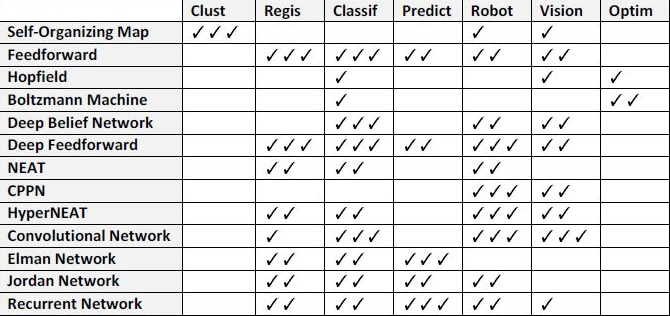
\includegraphics[scale=0.68]{images/typen_domains.png}
	\caption{Domänen zu Typen Matrix \cite{AI3}}
	\label{fig:DomainMatrix}
\end{figure}

Wie in der Abbildung \ref{fig:DomainMatrix} erkennbar ist, existiert kein Netzwerk Grundtyp, der für alle Problemdomänen geeignet ist.
Dies führt zu der Schlussfolgerung, dass je nach Aufgabe und Ziel ein entsprechendes Grundgerüst gewählt werden muss. 
Auf Basis dieses Grundgerüsts können uneingeschränkt weitere Eigenheiten aus anderen Netzwerken eingebaut werden.
In der Praxis findet man selten ein Netzwerk von einem Typ.
Meistens sind es einige mehrere Netzwerke unterschiedlicher Typen die hintereinander und parallel geschallten sind und so ein ganzen System darstellen.
Dabei übernimmt jedes Teilnetzwerk eine kleine Aufgabe des gesamten und zwar eine für die es Entwickelt wurde.
Aktuelle Netzwerke wie das Inception v3 Netzwerk von Google Research benötigt zwei Wochen mit acht Grafikkarten zum Trainieren. 
Ab diesem Zeitpunkt ist es im Stande akkurate Resultate zu liefern. 
Dieses Netzwerk ist sehr Komplex und besteht nicht nur aus 3 Ebenen, was zur Schlussfolgerung führt, dass um so tiefer das Netzwerk ist um so aufwändiger ist es zu Trainieren.

\section{Optimierung}

Optimierungen beinflussen das Lernverhalten und das Speicherverhalten eines Netzwerkes.

%Gegenmaßnahme -> dropout, Regulatoren 1/2, learnrate, momentum
\paragraph{Lernrate} skaliert die Lerngeschwindigkeit. 
Wie im Punkt Backpropagation \ref{sec:Backpropagation} beschrieben.

\paragraph{Momentum} gehört auch zur Optimierung im Algorithmus zur Backpropagation.
Dieser bestimmt wie stark frühere Gewichtsaktualisierungen berücksichtigt werden sollen. 

\paragraph{DropOut} gehört zur Kategorie der Regulatoren. 
Hinten (2012) beschreibt DropOuts als eine effektive Art, um Overfitting (siehe \ref{sec:AllgeProb}) zu vermeiden.
DropOut kann als System integriert werden aber auch als eigener Layer in einem Netzwerk.
In einem DropOutlayer werden immer Neuronen deaktiviert inklusive ihrer Verbindungen zu dem nächsten Layer.
Dies hat zur Folge, dass nur ein geringerer Teil an Informationen aus dem vorhergehenden Layer in den Nächsten übergehen. 
Durch diesen Prozess, des künstlichen gering halten der Informationen während dem Training führt dazu, dass das Netzwerk trotz dieser Einschränkung trotzdem versucht ein gutes Ergebnis zu erzielen. 
Während der Test- und Produktivphase werden diese DropOutlayer aber meist deaktiviert da das volle Potenzial des Netzwerks verwendet werden möchte.

\paragraph{L1 und L2 Regularisierung} sind auch Techniken die zur Verhinderung von Overfitting beitragen.
Im Gegensatz zu der DropOut Strategie sind diese zwei Regulationstechniken, Teil der Backpropagation oder Teil einer Funktion.
Beide Techniken arbeiten mit Strafen welche verteilt werden und so die Gewichtungen in ein Muster zwingen. 
%TODO objective functions -> simulated annealing
Im Falle von L1 ähnelt dieses Muster einer Gaussian Glockenkurve und bei L2 einer Laplace Kurve.
Durch das Bestrafen der Gewichtungen im Netzwerk werden diese Werte gering gehalten, sodass sie nicht ausarten. 
Wenn ein Gewicht Richtung $0$ geht, führt dies unweigerlich zu einem indirekten Ausschluss aus dem Netzwerk.
Das Netzwerk wird spärlicher und leichtgewichtiger was aber wiederum als Resultat hat, dass ein Rauschen in den Daten möglicherweise erkannt wird und ignoriert wird.

\begin{equation}
	E := \frac{\lambda}{n} \sum\limits_{w}|w|
	\label{eq:L1ErrorTerm}
\end{equation}

Die Funktion \ref{eq:L1ErrorTerm} bildet die Berechnung der Strafe in der Backpropagation ab.
Das $\lambda$ definiert wie stark die Regulierung den Error-Wert des Netzwerkes beeinflussen soll.
Ein Wert von $0$ führt dazu, dass die Regulierung keinen Einfluss besitzt. 
Im einem normalen Fall ist dieser Wert kleiner als $0.1 (10\%)$.
Der Divisor n wird durch die Anzahl an Elementen im Trainingssatz und der Anzahl an Neuronen im Outputlayer bestimmt.
Zum Beispiel bei $100$ Elementen im Trainingssatz und $3$ Neuronen im Outputlayer würde der Divisor den Wert $300$ einnehmen.
Dies ist erforderlich da diese Funktion bei jeder Evaluierung der Trainingsdaten berechnet wird.

\paragraph{GPU - GPGPU}

%\section{Tensorflow Typen Unterstützung}

\chapter{TensorFlow}
\label{cha:TensorFlow}

TensorFlow repräsentiert eine Bibliothek für Machine Intelligence. 
Historisch gesehen entstand TensorFlow in der Google Brain Abteilung.
Das Projekt wird als Open Source Projekt weiterentwickelt, wobei das Projekt von Google weiterhin gepflegt wird. 
Das Offenlegen des Projekts führt dazu, dass auch Personen außerhalb von Google die Möglichkeit bekommen, die Bibliothek zu verwenden sowie dazu etwas beitragen zu können. \newline

\noindent
Das Hauptkonzept in TensorFlow sind sogenannte Tensoren, welche einen Graphen durchlaufen. 
%Diese Tensoren werden während ihrem durch lauf verändert und wieder neu zusammengesetzt. 
Der Graphen selbst stellt damit einen Datenflussgraphen dar, welcher Knoten beinhaltet. 
Diese Knoten bilden numerische Operationen ab.
Der Informationsaustausch zwischen den Knoten geschieht mit multidimensionalen Arrays, den so genannten Tensoren.
TensorFlow bietet wie andere Bibliotheken die Möglichkeit die Berechnungen auf eine Grafikkarte auszulagern.
Zusätzlich sind weite Routinen eingebaut, damit das Trainieren über mehrere Grafikkarten verteilt werden kann sowie auf weitere Computer. \newline

\noindent
TensorFlow steht für mehrere Programmiersprachen zur Verfügung, welche offiziell unterstützt werden, wobei es noch mehr durch die Open Source Gemeinschaft unterstützte Sprachen gibt.
Den Hauptbereich stellt die Python API dar, welche auch die vollständigste Implementierung darstellt. 
Der Kern von TensorFlow ist mit C++ und Python implementiert und wurde sehr stark optimiert, um eine sehr gute Performanz zu erzielen.
Die Python API wird im Umfeld von TensorFlow dazu verwendet, um einen Graphen zu erstellen, zu trainieren und zu testen. 
Durch die Verwendung von Python besteht die Möglichkeit sehr schnell Änderungen am Graphen durchzuführen und nicht erst ganze Applikationsstrukturen zu übersetzten, damit ein Ergebnis der Änderung ersichtlich wird. 
Dieser Graphen wird nach seiner Trainingsphase exportiert und beinhaltet alle Knoten sowie die dazugehörigen Gewichtungen. 
Die C++ API sowie die Java API und GO API zielen auf eine sehr effiziente Ausführung ab.
Durch die Verwendung des trainierten Graphen kann dieser auch auf mobilen Plattformen eingesetzt werden.

\subsection{Graphs/Dataflowgraph}

\begin{figure}

\lstset{language=Python}
\begin{lstlisting}
import tensorflow as tf

b = tf.Variable(tf.zeros([100])) 
	# 100-d Vektor, initialisiert mit 0
W = tf.Variable(tf.random_uniform([784,100],-1,1)) 
	# 784x100 Matrix w/rnd vals
x = tf.placeholder(name="x") 
	# Platzhalter für Eingangsdaten
relu = tf.nn.relu(tf.matmul(W, x) + b) 
	# Relu(Wx+b) Aktivierungsfunktion mit impliziter Addition
C = [...] 
	# Kostenfunktion und noch weitere Knoten
s = tf.Session()
for step in xrange(0, 10):
	input = ...construct 100-D input array ... 
		# Erstellen eines 100-d Vektor mit den Eingangsdaten
	result = s.run(C, feed_dict={x: input}) 
		# Graphen mit den Eingangsdaten ausführen
	print step, result 
		# Ausgabe des Berechneten Resultats
\end{lstlisting}

	\caption{TensorFlow Codefragment zur Definition eines Teils des Graphen}
	\label{fig:SimpleFragmentGraphDefinition}
\end{figure}

\begin{figure}

	\centering

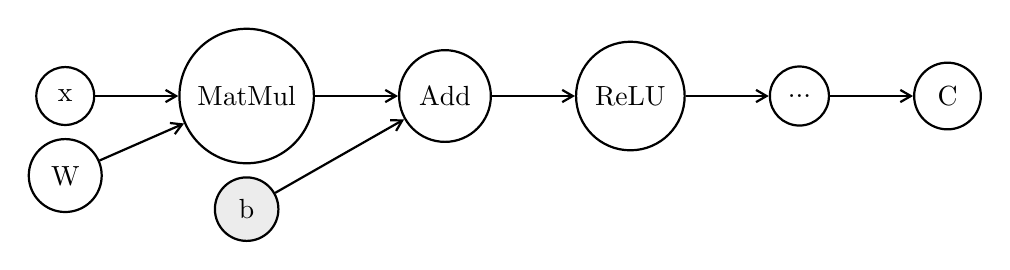
\begin{tikzpicture}

	\node[neuron] (x) {x};
	\node[neuron,below=of x] (w) {W};
	
	\node[group,fit={(x) (w)}] (gr1) {};
	
	\node[neuron,right=of x] (MatMul) {MatMul};
	\node[io,below=of MatMul] (b) {b};
	
	\node[group,fit={(x) (MatMul)},right=of x] (gr2) {};
	
	\node[neuron,right=of MatMul] (Add) {Add};
	
	\node[neuron,right=of Add] (ReLU) {ReLU};
	
	\node[neuron,right=of ReLU] (more) {...};
	
	\node[neuron,right=of more] (C) {C};
	
	\draw[conn] (x) -- (MatMul);
	\draw[conn] (w) -- (MatMul);

	\draw[conn] (MatMul) -- (Add);
	\draw[conn] (b) -- (Add);
	
	\draw[conn] (Add) -- (ReLU);
	\draw[conn] (ReLU) -- (more);

	\draw[conn] (more) -- (C);

\end{tikzpicture}

	\caption{Der resultierenden Teilgraph aus dem Codefragment aus Abbildung \ref{fig:SimpleFragmentGraphDefinition} nach dem Beispiel in \cite{wp2015tensorflow}}
	\label{fig:SimpleFragmentGraphPic}
\end{figure}

Ein TensorFlow Graph kann wie in Abbildung \ref{fig:SimpleFragmentGraphDefinition} beschrieben werden.
Dieser wurde zum Beispiel mit der Python API erstellt.
Im Gesamten mit den Knoten und den Verbindungen ergibt sich ein Datenfluss, diese beinhaltet alle erforderlichen Komponenten auch für das per sistieren und aktualisieren der Daten.
Dies sind Erweiterungen für den Hauptgraphen und beinhalten auch Logik für Schleifenverwaltungen.
Ein Knoten in einem Graphen besitzt $0$ bis $n$ Ein und Ausgänge und besitzt eine Kernfunktion. 
Zu den Datenhauptfluss mit den Tensoren gibt es zusätzlich spezielle Verbindungen, welche "control dependencies" genannt werden. 
Anhand dieser Verbindungen werden keine Daten im Sinne der Tensoren übertragen, sondern werden benützt um Abhängigkeiten zu definieren, um zum Beispiel eine Ausführung in einem anderen Knoten vor einem anderen zu definieren.
So muss der Quellknoten mit der Ausführung abgeschlossen haben bevor der darauf wartende mit der Ausführung beginnt. \cite{wp2015tensorflow}

\subsection{Operation}

Die Operation stellt in jedem Knoten den Kern dar, wie zum Beispiel eine Matrix Multiplikation oder eine Addition.
In TensorFlow selbst gibt es einen Unterschied zwischen Operation und Kernel.
Operationen besitzen Attribute, welche spätestens zum Zeitpunkt der Grapherstellung bekannt sein müssen. 
Ein solches Attribut wäre zum Beispiel, \textit{um eine Operation Polymorph für Datentypen zu ermöglichen}. 
Der Kernel selbst ist die Implementierung der Operation selbst. 
Dieser kann auf verschiedenen Geräten ausgeführt werden wie CPU oder GPU.
Die Operationen und die dazugehörigen Kernel werden über einen Registrierungsmechanismus zur Verfügung gestellt. 
Diese Sammlung an Operationen kann auch Erweitert werden. \cite{wp2015tensorflow} 

\subsection{Sessions}

Die Session repräsentiert die Laufzeit für einen Graphen. 
Dieser Session wird ein Graphen übergeben, welcher erst initialisiert werden muss. 
Ohne die Initialisierung ist der Knoten und Verbindungen würde die weitere Ausführung mit diesem nichts produzieren, da alle Werte $0$ sind. 
Diese stellt eine weitere Funktion zur Verfügung \textit{Run}. 
Der Run-Funktion wird eine Liste Endknoten übergeben welche berechnet werden sollen und die zu dem initialisierten Graphen gehören. 
Die Platzhalter Tensoren werden mit Daten verknüpft und so in den Graphen gereicht. 
In den Meisten fällen wird ein Graphen einmal erstellt und mehrfach ausgeführt. \cite{wp2015tensorflow} 

\subsection{Tensor}

In TensorFlow ist ein Tensor ein typisiertes multidimensionales Array. 
Die verwendbaren Typen reichen von Datentypen mit Vorzeichen und ohne sowie bis hin zu Doubles und Zeichenketten. \cite{wp2015tensorflow} 

\subsection{Hyperparameter} 

Hyperparameter werden im Umfeld von maschinellem Lernen verwendet, um Variationen an Kombinationen zu testen. 
Dabei werden verschiedenste Parameter getestet, wie verschiedene Aktivierungsfunktionen oder Optimierungsalgorithmen, aber auch die Anzahl an Ebenen und Breiten dieser. 
Im Gesamten führt dies meist zu sehr vielen Permutationen, welche ausgetestet werden müssen und somit voll trainiert werden. 
Da die Zeit welche dafür benötigt werden würde, nicht in einer Relation dazu steht, werden solche BroudForce Tests nur mehr selten durchgeführt. 
Für diesen Fall existieren eigene Techniken, welche sich nur um das Optimieren der Hyperparameter kümmern. \cite{bishop2006pattern}

\section{Bibliotheksinhalt}

\subsection{Datentypen}

TensorFlow besitzt eine große Anzahl an Datentypen die verwendet werden können. 
Dies reicht von Grunddatentypen wie 'Boolean' und 'String' bis hinzu verschiedene Integer Datentypen. 
Diese stehen in verschiedene Wertebereichen zur Verfügung. 
So gibt es Gleitkommazahlen mit unterschiedlicher Genauigkeit, wie 16-bit was für halbe Genauigkeit steht aber auch bis zu 64-bit Genauigkeit reicht, was einer doppelten Genauigkeit entspricht. 
Der Grund für diese verschiedenen Anzahlen an Datentypen ist, dass diese zur Optimierung verwendet werden können. 
Ein trainiertes Netzwerk welches nie in den Wertebereich von 64-bit signierte Integers gekommen ist, wird diese möglicherweise nie benötigen. 
In diesem Fall können die Wertebereiche reduziert werden, auf zum Beispiel 32-bit signierte Integer und somit die Berechnungen hochperformanter ausgeführt werden. \cite{TensorFlow}

\subsection{Operationen}

\subsubsection{Konstanten und Zufallswerte}

\paragraph{Konstanten} stehen in TensorFlow vordefiniert zur Verwendung.
Diese stellen initialisierte Tensoren für den ersten Trainingsdurchlauf zur Verfügung.

\begin{itemize}
	\item \textit{tf.zeros} erstellt einen Tensor mit angegebenen Dimension bestehend aus $0$ und von einem Datentypen. 
	\item \textit{tf.zeros\_like} gibt einen Tensor zurück, welcher die selbe Dimensionen wie der gegeben besitzt.
	Alle Werte in diesem Tensor sind aber auf $0$ gesetzt.
	In diesem Zuge kann der Datentyp mit angepasst werden, wenn nur die Dimensionen übernommen wenden sollen.
	\item \textit{tf.ones} agiert genau wie der Tensor \textit{tf.zeros} mit dem unterschied dass alles mit $1$ gefüllt ist.
	\item \textit{tf.ones\_like} repräsentiert das selbe wie \textit{tf.zeros\_like} nur mit $1$.
	\item \textit{tf.fill} wird zu der Dimension noch ein Skalar mit gegeben, für die Werte die ausgefüllt werden sollen.
	\item \textit{tf.constant} liefert einen Tensor mit selbst definierbaren Werten. 
	Diese Werte können eine Liste sein sowohl als auch eine einzelner Wert welcher überall eingefügt werden soll. 
\end{itemize}

\paragraph{Sequenzen} können verwendet werden um einen Wertebereich in eine bestimmte Anzahl an Werte zu zerteilen und diese als Tensor in das System einfließen zu lassen.

\begin{itemize}
	\item \textit{tf.lin\_space} generiert einen eindimensionalen Tensor vom Datentypen $32$ oder $64$-bit Gleitkommazahlen, mit einer bestimmten Folge.
	Diese beginnt mit dem Startwert und endet mit dem Endwert. 
	Die Werte dazwischen werden gleichmäßig verteilt erstellt. 
	\item \textit{tf.range} erstellt wie \textit{tf.lin\_space} einen eindimensionalen Tensor mit Skalarwerten. 
	Die Folge beginnt mit einem Startwert und erweitert sich um ein Delta bis zum Endwert, welcher nicht Teil der Folge ist. 
\end{itemize}

\paragraph{Zufallswerte} werden im Bereich von maschinellen Lernens sehr häufig benötigt. 
So werden meist der Startzustand mithilfe von Zufallszahlen hergestellt. 

\begin{itemize}
	\item \textit{tf.random\_normal} liefert einen Tensor mit Zufallswerten anhand einer Normalverteilung (Gaussian). 
	Die Dimension des Ergebnistensors muss spezifiziert werden, der Meridian, Standardabweichung sowie der resultierende Datentyp können angegeben werden. 
	\item \textit{tf.truncated\_normal} verhält sich gleich zu \textit{tf.random\_normal} mit dem unterschied, dass Werte die größer sind als $2$-mal die Standardabweichung, ignoriert werden und ein neuer Wert ausgewählt wird.
	\item \textit{tf.random\_uniform} generiert einen Tensor in welchem Werte gleich Wahrscheinlich vorkommen.
	Die Werte werden aus dem spezifizierten Wertebereich genommen, wobei diese exklusive der oberen Grenze ist, wie zum Beispiel '$[0, 1)$'.
	\item \textit{tf.random\_shuffle} erstellt selber keine neuen Werte sondern, mischt einen Tensor anhand seiner ersten Dimension durch. 
	\item \textit{tf.random\_crop} liefert einen zufälligen Teil eines Tensors mit der selben Anzahl an Dimensionen und aber mit der spezifizierten Größe.
\end{itemize} \phantom \newline

\noindent
Einige dieser Funktionen benötigen sogenannte Seed-Werte, welche den Startwert der Zufallszahlen zerstreuen sollen sowie die Folge selbst. 
Im Falle von TensorFlow beruht dies auf zwei Werten, einer wird für den Graphen spezifiziert, der zweite wird für die Operation selbst spezifiziert. 
Der Wert für den Graphen kann mit \textit{tf.set\_random\_seed} gesetzt werden. 
Für weiter Informationen steht die online Dokumentation zur Verfügung. \footnote{Online Dokumentation: Constants, Sequences, and Random Values  \url{https://www.tensorflow.org/api_guides/python/constant_op}}

\subsubsection{Variables}

Variablen geben bei jedem Durchlauf einen Tensor ab.
Dieser Wert ändert sich nicht, außer ihm wird eine neuer Wert zugewiesen. 

\subsubsection{Transformationen}

\paragraph{Casting} bietet die Möglichkeit wie in anderen Programmiersprachen Typen zu konvertieren. 
Diese Operation muss in den Graphen eingepflegt werden, da keine impliziten Konvertierungen durchgeführt werden. 
Es kann jeder Tensor konvertiert werden, sowie eine Zeichenfolge in eine Zahl. 
Bei diesem Vorgang kann ein Fehler entstehen, welcher in \textit{TypeError} resultiert.

\paragraph{Shapes und Shaping} liefert die Gestalt eines Tensors, bietet aber auch die Möglichkeit diese zu ändern. 
\begin{itemize}
	\item \textit{tf.shape} liefert eine genaue Aufschlüsselung des Tensors mit der Dimension und der Tiefe.
	\item \textit{tf.size} repräsentiert die Anzahl an Elementen in einem Tensor. 
	Diese Anzahl ergibst sich aus den konkreten Werten.
	\item \textit{tf.rank} verhält sich ähnlich zu \textit{tf.size} mit dem unterschied, dass die Anzahl der Felder Vertiefung gezählt wird.
	\item \textit{reshape} wird verwendet um Tensoren in eine neue Struktur zu bringen. 
	Dabei kann für das einebnen der Dimensionen eine Kurzschreibweise verwendet werden mit $-1$ als Zielausführung der Gestalt.
	\item \textit{tf.squeeze} entfernt ganze Dimensionen aus dem gegebenen Tensor. 
	Ohne Achsen Angabe werden alle Dimensionen mit der Größe $1$ entfernt oder es werden die spezifizierten Dimensionen herausgenommen.
	\item \textit{tf.expand\_dims} gliedert wider um Dimensionen in einen Tensor ein. 
	Im Standard an der Indexstelle $0$, außer es wurde spezifiziert.
\end{itemize}

\paragraph{Slicing und Joining} wie in diversen Programmiersprachen unterstützt auch TensorFlow das Teilen und Zusammenfügen von Daten und aber hier im Speziellen mit Tensoren. 
Diese Operationen reichen von einfachen Slicing Operationen über Transponieren bis hin zu dem Verketten von Tensoren, dabei kann definiert werde Anhand welcher Achse der Dimensionen die Operation ausgeführt werden soll.

%\paragraph{Fake quantization} => zu viel
\phantom \newline

\noindent
Weiter Informationen befinden sich in der online Dokumentation. \footnote{Online Dokumentation: Tensor Transformations \url{https://www.tensorflow.org/api_guides/python/array_ops}}

\subsubsection{Mathematik} 

\paragraph{Arithmetische Operationen} stellen die mathematischen Grundoperationen dar. 
Diese können teilweise in Kurzschreibweisen verwendet werden, wie zum Beispiel die Addition. 
Diese kann entweder als explizite Operation \textit{tf.add(x, y)} verwendet werden aber auch Implizit bei der Addition $+$ von einem Tensor mit einem Bias-Tensor.

\paragraph{Basis Funktionen} ergänzen die arithmetischen Operationen um Standardfunktionen. 
Zu diesen Funktionen zählen die Berechnung der Absolutwerten in einem Tensor sowie eine Exponentialfunktion. 

\paragraph{Matrizen Funktionen} werden am häufigsten benötigt, da Tensoren im Grunde Matrizen sind und somit diese geändert werden können. 
\begin{itemize}
	\item \textit{tf.matmul} führt eine Matrizenmultiplikation aus. 
	Diese Operation findest meist in voll Vernetzten Neuronen Verwendung, wenn der übergebene Tensor mit der Gewichtung multipliziert wird. 
	\item \textit{tf.eye} erzeugt eine Identitätsmatrix, in welcher alle Werte an der Diagonale $1$ sind und alle anderen $0$. 
\end{itemize}

Zu diesen Funktionen existieren noch weitere die zur Lösung von Gleichungen verwendet werden können. 
Diese Gleichungen müssen in Matrizenschreibweise im Tensor abgebildet sein. 

\paragraph{Komplexe Zahlen} können verwendet werden und Operationen mit ihnen in de Graphen eingepflegt werden. 

\paragraph{Reduzierungsoperationen} kommen meist dann zum Einsatz, wenn der Unterschied zwischen dem Ergebnis und dem erwarteten Ergebnis festgestellt werden soll. 
\begin{itemize}
	\item \textit{tf.reduce\_sum} berechnet die Summe aller Werte in einem Tensor.
	\item \textit{tf.reduce\_mean} berechnet die Summe aller Werte an der Diagonale eines Tensors. 
	\item \textit{tf.reduce\_max} reduziert einen Tensor auf die maximal Werte in der letzten Dimension und reduziert dabei den Rang um eins.
\end{itemize}

\noindent
Zu diesen gibt es noch weiter, welche in diversen Fällen benötigt werden wenn zum Beispiel Wahrheitswerten reduziert werden sollen. \newline

\noindent
Die Anzahl an mathematischen Funktionen ist um einiges sehr viel Größer als die hier erwähnten. 
Diese hier repräsentieren lediglich die meist verwendeten Operationen. 
Für weiter Informationen steht die online Dokumentation zur Verfügung. \footnote{Online Dokumentation: Math \url{https://www.tensorflow.org/api_guides/python/math_ops}}

\subsubsection{Flusskontrolle}

\paragraph{Flusskontrolle} sind Operationen die den Ablauf in dem Graphen beeinflussen. 
Dies können Bedingungen sein, wie im Sinne von \textit{if (Bedingung){...} else {}} aber auch \textit{switch (Term) { case '0': ...; break;}} Bedingungen sein. 
In beiden Fällen müssen die Auszuführenden Verzweigungen als Funktionen vorliegen. 
Zusätzlich gibt es noch eine \textit{While} und eine \textit{For} Schleife. 
Zu beachten ist, dass diese Operationen und weiter den Fluss durch den Graphen stark beeinträchtigen können.

\paragraph{Logik Operatoren} können verwenden werden um Vergleiche zwischen Tensoren durchzuführen. 
Diese werden aber als Logik Operationen ausgeführt und liefern immer Wahrheitswerte, wie eine Logische Und-Verknüpfung auf Binärebene.

\paragraph{Vergleichsoperatoren} neben den Logischen Operatoren stehen weitere Vergleichsoperatoren zur Verfügung. 
Hierzu zählen \textit{tf.equal} sowie die verneinte Variante, \textit{tf.less} und \textit{tf.greater} mit jeweils einer gleich Version. 
Diese Operatoren geben wiederum einen Tensor mit Wahrheitswert aus.

\paragraph{Debugging Operationen} ermöglichen es in den Graphen Kontrollstrukturen einzubauen, welchen auf diverse Bedingungen reagieren.
So kann Überprüft werden ob ein Tensor Werte mit undefinierten Zustand beinhaltet. 
Die Funktion \textit{tf.Print} ermöglicht es Tensoren auszugeben wenn diese Funktion im Graphen evaluiert wird. 
Aktuell sind die Möglichkeiten eine Graphen zu debuggen relative eingeschränkt, da der Graphen ist grundsätzlich einsehbar aber schwer zu verstehen in seiner rohen Darstellung.
\footnote{Online Dokumentation: Control Flow \url{https://www.tensorflow.org/api_guides/python/control_flow_ops}}

\subsubsection{Images}

\paragraph{Encodieren und Decodieren} von Bilddateien wird TensorFlow direkt unterstützt.
Dabei können Bildern von den Datentypen Gif, Jpeg und PNG gelesen werden, sowie das erstellen von Bildern in diese Datentypen, ausgenommen Gif. 
In allen Fällen wird das Bild als Zeichenkette mit Pfad angegeben. 

\paragraph{Größenänderung} von Bilder sind erforderlich, da Bilder die eingelesen werde zu große sind und somit in die Struktur des Graphen nicht eingelesen werden können. 
Für die Größenänderung stehen mehrere Implementierungen zur Verfügung mit unterschiedlichen Algorithmen und vorgehen im Hintergrund.

\paragraph{Beschneiden} wird dann benötigt wenn aus einem Bild ein Teil herausgenommen werden soll. 
Zum herausnehmen stehen wiederum mehrere Operationen zur Verfügung, welche mit umschließende Boxen arbeiten oder wie viel Prozent von der Mitte des Bildes aus genommen werden soll.

\paragraph{Flippen, Rotieren und Transponieren} ermöglicht es Bilder zu Verändern, so dass es für einen Menschen mehr oder weniger immer noch die selbe Bedeutung hat aber nicht mehr für einen Computer. 
Für diesen stellt ein Rotiertes oder Gespiegeltes Bild ein neues Bild dar. 
Diese Technik wird beim Trainieren von Bilderkennungen eingesetzt um zum Beispiel aus geringen Datenmengen die zum Trainieren verfügbar sind, mehrere zu generieren.
\phantom \newline

\noindent
Zusätzlich gibt es noch die Möglichkeit die Farbkanäle des Bildes zu ändern sowie das Bild nachzujustieren. 
\footnote{Online Dokumentation: Images \url{https://www.tensorflow.org/api_guides/python/image}}

\subsubsection{Input und Readers}

\paragraph{Platzhalter} werden benötigt um einen Graphen zu erstellen. 
Ohne Platzhalter wäre es nicht möglich Daten in den Graphen zu bekommen. 
Diese müssen zur Ausführungszeit durch richtige Daten ersetzt werden, was mit Hilfe von einem Schlüssen-Wert-Paars erfolgt. 

\paragraph{Readers} ermöglichen direkt aus dem Dateisystem Daten zu laden. 
Dabei stehen spezifizierte Reader zur Verfügung welche die direkt Tensoren ausliefern sowie Zeile für Zeile  oder ganze Dateiinhalte liefern. 

\paragraph{Konvertierungsoperationen} ermöglichen es Dateien die mit TensorFlow Readers gelesen wurden weiter zu verarbeiten, so kann eine CSV Datei decodiert verwendet werden.
\phantom \newline

\noindent
Des Weiteren sind Protokoll Buffer sowie Queues implementiert die zum Vorverarbeiten von Daten sind.
\footnote{Online Dokumentation: Input und Readers \url{https://www.tensorflow.org/api_guides/python/io_ops}}

\subsubsection{Neuronale Netzwerke}

Neuronale Netzwerke sind eine Spezialisierung des Gebietes des maschinellen Lernens. 
So bietet TensorFlow eine breite Unterstützung beziehungsweise eine große Implementierungsvielfalt für diesen Typ an. 

\paragraph{Aktivierungsfunktion} repräsentieren den Ausgang eines Neurons dar, dabei existieren aus der Vergangenheit heraus einige Ansätze für diesen Bereich eines Neuronalen Netzwerkes. 
\begin{itemize}
	\item \textit{tf.sigmoid} ist eine der bekanntesten und ältesten diesen Typs.
	Diese Funktion hat im Punkt $0$ einen Aktivierungswert von $0.5$ und besitzt zwei Beschränkungen. 
	Im negativen Zahlenbereich auf der X-Achse wird die Funktion mit $0$ der Grenzwert definiert und im positiven Zahlenbereich auf der X-Achse wird diese mit dem Grenzwert von maximal $1$ definiert. 
	Ein negativer Wert führt somit zu einem geringen Aktivierungswert, welcher sich im Negativen an $0$ annähert sowie im Positiven an $1$.
	Im Diagramm \ref{fig:Sigmoide Aktivierungsfunktion} befindet sich dies Funktion mit ihren Grenzwerten. 
\begin{figure}
	\centering
	\resizebox {\linewidth} {5cm} {
	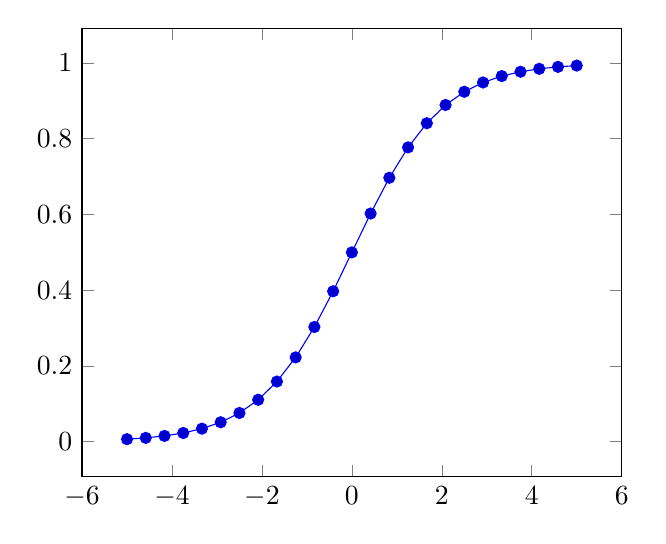
\begin{tikzpicture}
	\begin{axis}

		\addplot expression { 1/(1+exp(-x) };

	\end{axis}
	\end{tikzpicture}
	}
	\caption{Sigmoide Aktivierungsfunktion}
	\label{fig:Sigmoide Aktivierungsfunktion}
\end{figure}

	\item \textit{tf.relu} ersetzt mittlerweile immer mehr die Sigmoide Version. 
	Ein Grund dafür ist, dass die Berechnung mit Sigmoidefunktionen Ressourcen intensive ist. 
	Die rektifiziert lineare Funktion ist sehr viel einfacher, denn Werte unter $0$ werden als $0$ weiter gegeben und Werte darüber linear. 
	Somit resultiert ein Eingangswert von $-0.1$ in einer $0$ und ein Wert von $0.5$ in $0.5$.
	Wie im Diagramm \ref{fig:rektifiziert lineare Aktivierungsfunktion} ersichtlich ist, führt dies bei einem negativen Wert dazu, dass eine Multiplikation mit der Gewichtung in der nächsten Ebene ebenfalls in einer $0$ sich repräsentiert und somit in der Addition ignoriert wird.
\begin{figure}
	\centering
	\resizebox {\linewidth} {5cm} {
	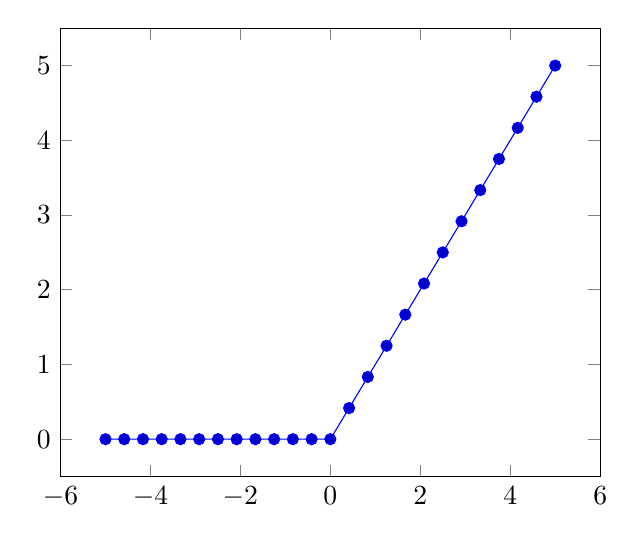
\begin{tikzpicture}
	\begin{axis}

		\addplot expression { max(0, x)};

	\end{axis}
	\end{tikzpicture}
	}
	\caption{rektifiziert lineare Aktivierungsfunktion}
	\label{fig:rektifiziert lineare Aktivierungsfunktion}
\end{figure}

	\item \textit{tf.tanh} genannt als Hyperbolic Tangent gehört ebenfalls zu den grundlegenden Aktivierungsfunktionen. 
	Der Unterschied zwischen dieser Funktion und der Sigmoiden Aktivierungsfunktion ist, dass der untere Grenzwert nicht bei $0$ liegt sondern bei $-1$. 
	Im Diagramm \ref{fig:Hyperbolic Tangents Aktivierungsfunktion} ist zu sehen, wo sich der Wendepunkt befindet, was im Falle des Hyperbolic Tangent in der Koordinate $x = 0, y = 0$ ist. 
\begin{figure}
	\centering
	\resizebox {\linewidth} {5cm} {
	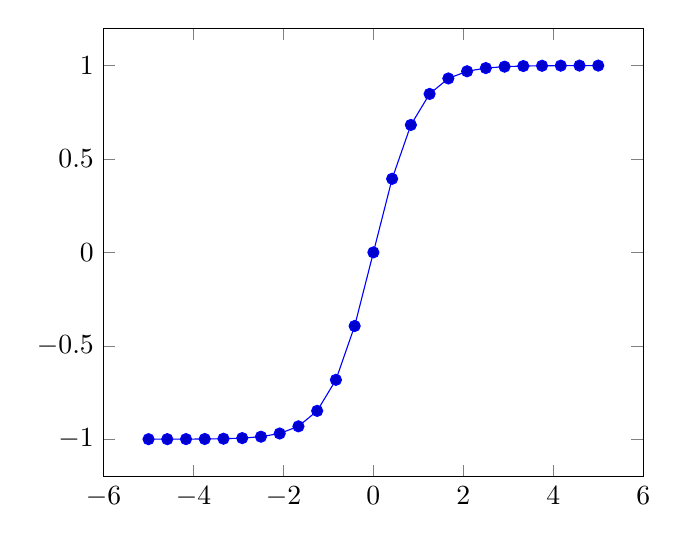
\begin{tikzpicture}
	\begin{axis}

		\addplot expression { tanh(x)};

	\end{axis}
	\end{tikzpicture}
	}
	\caption{Hyperbolic Tangents Aktivierungsfunktion}
	\label{fig:Hyperbolic Tangents Aktivierungsfunktion}
\end{figure}
\end{itemize}
\phantom \newline

\noindent
Zu diesen Aktivierungsfunktion stehen noch einige weiter zur Verfügung, die ausführlich getestet gehören. 
Im Grunde könnte jede Funktion verwendet werden, doch jede besitzt eine Eigenheit und beeinflusst so den gesamten Graphen. 

\paragraph{Faltung Operationen} werden bei Bilderkennungen unter anderem deshalb verwendet, da sie eine Operation auf einen Stapel an Daten gleichzeitig anwenden. 
So wird wird ein Fenster über ein Bild geschoben und auf jedes Bild wird in dem selben Fenster die Operation durchgeführt. 
Diese Operation generalisiert die darunterliegenden Daten, so als ob sie auf Etwas reagiert hätten. 
Dies entspricht dem als ob ein Auge auf etwas reagiert hätte. 
\textbf{TODO: Diagramm}
\begin{itemize}
	\item \textit{tf.nn.conv2d} steht für zweidimensionale Bilder zur Verfügung. 
	\item \textit{tf.nn.conv3d} ermöglicht es mit dreidimensionale Objekte zu arbeiten.
\end{itemize}
\phantom \newline

\noindent
Des Weiteren stehen noch weitere spezialisierte Versionen implementiert zur Verfügung.

\paragraph{Bündelung} wird verwendet um Daten zu vereinfachen. 
Eine Faltungsoperation führt dazu, dass aus einem Bild viel erzeugt werden mit unterschiedlichen Filtern. 
Eine Bündelung ermöglicht einen Vereinfachung der Bilder, sodass sie vereinfacht werden und dabei die Schlüsselinformationen aber dennoch erhalten bleiben. 
Diese Technik wurde zu früheren Zeiten eingesetzt, um Computerressourcen zu sparen, da diese nicht so leistungsfähig waren wie sie aktuell sind. 
TensorFlow bietet mehrere Umsetzungen, so kann der Maximalwert aus der Filtermatrix übernommen werden wie aber auch der Mittelwert. 

\paragraph{Verluste} beschreiben wie sehr ein Ergebnis von dem erwarten Ergebnis entfernt ist. 
Diese Art der Verlust Feststellung wird bei Regression Probleme benötigt aber auch regulieren im generellen.
\begin{itemize}
	\item \textit{tf.nn.l2\_loss} berechnet einen Wert, welcher den Inhalt des Tensors repräsentiert. 
	Im Falle dieser Implementierung wird keine Wurzel des Quadrats berechnet, sondern es werden die Werte nur addiert und durch $2$ dividiert.
	\item \textit{tf.nn.log\_poisson\_loss} berechnet den Logarithmischen-Wahrscheinlichkeitsverlust zwischen einem Ergebnis und einem erwarteten Ergebnis. 
	Diese Methode liefert im Normalfall nicht den exakten Verlust, was für Optimierungen nicht das Problem ist. 
	Sollte trotzdem ein genaueren Wert berechnet werden zum Vergleichen von Verlusten, muss die aufwändige Stirling Approximation aktiviert werden. 
\end{itemize}

\paragraph{Klassifizierungen} repräsentieren eine großen Bereich des maschinellen Lernens. 
TensorFlow besitzt deshalb mehrere Hilfsfunktionen, welche das arbeiten mit Klassifizierungen erleichtert. 
\begin{itemize}
	\item \textit{tf.nn.softmax} bildet alle Ergebnisse auf einen prozentualen Bereich ab. 
	So ergeben alle möglichen Ausgänge in Summe 100\%, was soviel bedeutet das ein Ergebnis eine gewisse Wahrscheinlichkeit besitzt. 
	\item \textit{tf.nn.softmax\_cross\_entropy\_with\_logits} bietet einem die Möglichkeit auf nicht skalierte Daten ein Ergebnis zu Berechnen, welches eine \textit{tf.nn.softmax} Berechnung liefern würde. 
	Zusätzlich wird eine weitere so genannte 'cross entropy' Operation ausgeführt, wo das Ergebnis für Optimierungen benötigt wird. 
	Die gesamte Methode berücksichtigt Spezialfälle im gesamten Prozess, welche schwer manuell ab zu berücksichtigen sind. 
\end{itemize}
\phantom \newline

\noindent
Zu diesen existieren noch weitere Implementierungen mit weiteren Eigenheiten, welche in diversen Situation möglicherweise einen Vorteil bieten. 

%\paragraph{Wiederkehrend Neuronale Netzwerke} 

\noindent
Des Weiteren gibt es Implementierungen für Wiederkehrende Neuronale Netzwere und weiter Dinge in diesem Themengebiet. 
\footnote{Online Dokumentation: Neural Network \url{https://www.tensorflow.org/api_guides/python/nn}}

\subsubsection{Running Graphs}

\paragraph{Session} stellt eine Hauptklasse des TensorFlow-Systems dar, mit der TensorFlow Engine im Hintergrund.
In ihr werden alle Operationen ausgeführt und alle Tensoren evaluiert. 
Dieser Session wird der Graphen mitgegeben, in dem der Endpunkt des Graphen angeben wird. 
Zur Ausführungszeit führt die Engine alle Operationen des Graphen durch und evaluiert die Tensoren in diesem. 
Die Engine führt dabei alles bis zu dem gegebenen Punkt aus, welcher als Ausgangspunkt übergeben wurde. 
Sollte der Graphen weiterführen, so wird dieser nicht mehr durchlaufen. 
Dies bietet eingeschränkte Möglichkeit, um das aufgebaute System zu testen. 
Eine Session wird mit \textit{tf.Session} erstellt und stellt die Funktionalität zum Ausführen, sowie die Möglichkeit diese zu schließe zur Verfügung. 
Mit \textit{tf.InteractiveSession} wird ebenfalls eine Session erstellt, diese wird aber zugleich als Basissession installiert. 
Dies bietet die Möglichkeit interaktive in einer Kommandozeile Operationen auszuführen, ohne die Session expliziert zu übertragen und anzusprechen. 
Die Tensoren und Operatoren bietet in diesen Fall die Option sich und den Graphen auszuführen, indem die Methoden \textit{TensorVariable.eval} sowie \textit{OperationsVariable.run} in diesen Aufgerufen werden. 

\noindent
Zusätzlich kann eine bestehende Basissession geholt werde sowie auf Fehler reagiert werden. 
\footnote{Online Dokumentation: Running Graphs \url{https://www.tensorflow.org/api_guides/python/client}}

\subsubsection{Training}

\paragraph{Optimizers} stellen einen weiteren Kernteil des System dar. 
TensorFlow stellt einen Menge an implementierten Optimierungsalgorithmen zur Verfügung. 
Diese Operationen trainieren den Graphen mit der gewählten Technik des gewählten Algorithmus. 
Diese Implementierungen versuchen die gegebenen Kosten eines Graphen zu minimieren. 
Bei der Verwendung von \textit{minimize} führt die Operation zwei Schritte in einem aus. 
In diesem wird der Gradient berechnet und dieser wird direkt auf die Variablen adaptiert. 
Diese Schritte können in einzelne zerlegt werden wenn, sollte mit den berechneten Gradient noch etwas zusätzlich durchgeführt werden. 
Die Berechnung wird dabei mit \textit{opt.compute\_gradients} ausgelöst, was einen Liste mit Paaren liefert. 
Diese Liste kann bearbeitet werden aber auch zu Testzwecken mit Protokolliert werden. 
Die Gradienten werden in dritten Schritt mit \textit{opt.apply\_gradients} auf die Variablen angewendet. 
Jeder Optimierungsalgorithmen verfügt über Eigenheiten und spezielle Verhalten, welche berücksichtigt werden sollten bei der Auswahl des Optimierers.

\paragraph{Gradient Computation} umfasst Methoden die das Verhalten des Graphen und der Optimierung beeinflussen. 
Diese Methoden ermöglichen es, Einfluss auf die Gradientenberechnung sowie auf dessen Evaluierung zunehmen. 
In diesem Sinne sind diese mit Vorsicht zu verwenden.

\paragraph{Verteilte Ausführung} stellt eine der Stärken von TensorFlow dar, da diese Technologie schon im System implementiert ist und somit keine manuelle Verteilung der Aufgaben entwickelt werden muss.
Dadurch besteht die Option die Berechnungen auf mehrere Geräte zu verteilen und so die zur Verfügung stehenden Ressourcen besser auszunützen. \\
%Im Grunde wird ein Cluster definiert welcher Computerknoten umfasst. 
%Diesen werden dann Tasks auf Aufgaben zugewiesen, wobei zu den Knoten definiert werden muss was zu tun ist.

\noindent
Einige Komfortmethoden ermöglichen es einfacher eine Session zu erstellen und alle Variablen zu initialisieren, sowie im Anschluss zu trainieren, wobei eine Stopbedingung mit definiert werden kann.
In diesem Zuge können Hooks einfach in das System integriert werden welche Aufgerufen werden.

\noindent
Im Weiteren kann Threading sowie der Verfall der Lernrate beeinflusst werden.
\footnote{Online Dokumentation: Training \url{https://www.tensorflow.org/api_guides/python/train}}

%\subsection{Probleme}

%\subsubsection{NaN Problem}

TensorFlow beinhaltet noch sehr viele weiter Komponenten und Möglichkeiten. 
Dies würde aber den Rahmen und den ersten Einblick in die Materie des maschinellen Lernens und im speziellen von TensorFlow sprengen. 
Im Grunde kann mit diesem Grundlagen und ein Netzwerk erstellt werden und damit gearbeitet werden. 
Seit der Offenlegung kommen immer mehr Erweiterungen aus der Community dazu, was auch dazu führt, dass Teile die sehr oft benötigt werden und aus mehreren Komponenten bestehen als Modul oder Funktion zur Verfügung stehen. 
Im Zuge dessen besteht die Möglichkeit sich einen bestehen Graphen zu nehmen, welcher zum Teil schon vor trainiert worden ist. 
Im Zuge dessen werden nur mehr die letzten Ebenen des Graphen trainiert und auf die konkrete Aufgabe hin ausgelegt. 
Dies hat zur Folge, dass schneller ein verwendbarer Graphen vorhanden ist, dieser aber sehr wahrscheinlich nicht der Beste ist den es geben würde. 

\subsection{TensorBoard}

TensorBoard stellt eine Erweiterung des TensorFlow-System dar, im Sinne einer Toolerweiterung. 
Jeder Graph kann in ein File Serialisiert werden, welches als Event-File bezeichnet wird. 
Dies hat zur Folge, dass dieser auch wieder geladen werden kann. 
Bei dieser Serialisierung werden alle Informationen des Graphen inklusive der Gewichtungen in die definierte Datei gespeichert.
TensorBoard bietet nun die Möglichkeit diesen Graphen zu laden und diesen Visualisiert darzustellen.
Zu den Graph-Informationen kann jeder Tensor mit gespeichert werden und als Diagramm visualisiert werden, mit einer zeitlichen Komponente. 
Dies ermöglicht es einem den Verlauf des Trainings zu analysieren. 
Aus einem Graphen können mehrere dieser Event-Files erzeugt werden sowie fixe Punkte definiert werden. 
Beim Laden eines Graphen in die TensorFlowt sowie TensorBoard-Umgebung kann spezifiziert werden zu welchen Zeitpunkt geladen werden soll. 
Damit wird ermöglicht viele Trainingsdurchläufe zu durchlaufen und bei einer Verschlechterung der Präzision zu einem früheren Zustand zurück zu springen.
Diese Tool ermöglichte es einem in das Verhalten eines Graphen ein wenig Einsicht zu nehmen und so die sogenannte Black Box zu durchleuchten. 

\paragraph{Namesbereiche (\textit{tf.name\_scope})} stellen eine Hilfe für die Darstellung und die Lesbarkeit des visualisierten Graphen dar. 
Durch die Verwendung des Python-Schlüsselwortes \textit{with} wird eine Ressource verwaltet und wieder freigegeben. 
In Verwendung mit \textit{tf.name\_scope} werden alle Operationen und Tensoren in diesem Block in der Visualisierung in einen benannten Block zusammengefasst.

\begin{figure}

\lstset{language=Python}
\begin{lstlisting}
import tensorflow as tf

with tf.name_scope("func"):
	b = tf.Variable(tf.zeros([100])) 
	W = tf.Variable(tf.random_uniform([784,100],-1,1)) 
	x = tf.placeholder(name="x") 
	relu = tf.nn.relu(tf.matmul(W, x) + b) 

C = [...] 
s = tf.Session()
for step in xrange(0, 10):
	input = ...construct 100-D input array ... 
	result = s.run(C, feed_dict={x: input}) 

	print step, result 
\end{lstlisting}

	\caption{TensorFlow Codefragment zur Namescope Verwendung in Graphen}
	\label{fig:NameScopeFragmentGraphDefinition}
\end{figure}
\phantom \newline

\noindent
Wie in der Codefragment \ref{fig:NameScopeFragmentGraphDefinition} beschrieben werden die Tensoren und Operatoren \textit{b, W, x, relu} in einen Block zusammen gefasst. 
In diesem Beispiel gibt es keinen Tensor, welcher in den Block übergeben wird, da die Daten in der Ausführung von außerhalb es System in dieses gelangen. 
Die Operation \textit{relu} und der daraus resultierende Tensor bilden den Ausgang des Blockes. 
Diese Technik der Namensbereiche ermöglicht es einem den Graphen zu strukturiere, da nicht wie in \textit{tf.zeros([100])} viele einzelne Knoten dargestellt werden, sonder abstrahiert werden und aber weiterhin einsehbar sind.

\paragraph{Graph} bildet den Punkt zum Visualisieren des Graphen selbst. 
Hierbei werden aus dem Event-File alle Informationen zum Aufbau des Graphen geladen und visualisiert. 
Durch die Verwendung der Namensbereichen werden Gruppen gebildet was dazuführt, dass die Gruppierungen möglicherweise in Ebenen sich widerspiegeln. 
Der dargestellte Graphen kann nach dem Einlesen und generieren interaktive Analysiert werden. 
So können Bereiche vergrößert und geöffnet werden und die definierten Tensoren betrachtet werden. 
Dieses Tool bietet zusätzliche Funktionalitäten, wie das das Darstellen wo am meisten Rechenzeit benötigt wurde sowie auch welche Berechnung auf welchem Gerät ausgeführt worden ist. 
Alle diese zusätzlichen Funktionalitäten benötigen Daten, welchen beim Erstellen des Graphen mit definiert werden müssen und auch mit in des Event-File serialisiert werden müssen. 

\paragraph{Event} repräsentiert den Bereich in welchem die Lernergebnisse dargestellt werden. 
Dies umfasst die Präzision sowie die Verluste. 
Das Ziel des Graphen ist im Grunde immer die Präzision zu erhöhen und die Verluste zu minimieren. 
Aus diesem Grund sollte sich die Genauigkeit an $1$ annähern, außer die Definition dieser Berechnung liefert andere Werte oder besitzt einen anderen Grenzwert. 
Der Verlust sollte sich im laufe des Trainings an $0$ annähern, denn dadurch spiegelt sich die Fehlerquote ab. 
Dies hängt aber wieder von dem entwickelten Graphen ab und kann sich somit einem anderen Wert annähern.
\phantom \newline 

\noindent
Event bietet die Möglichkeit mehrere Graphen und ihre Eventdaten zu visualisieren. 
In diesem Fall werden alle gelesen Events in einer Liste aufgelistet, in welcher ausgewählt werden kann welche Ausführung in den Diagrammen dargestellt werden sollen. 
In diesem Zuge können diese Diagramme zusammen geführt werden und so die Ergebnisse direkt verglichen werden. 
Dies hat den Vorteil, dass ein Netzwerk mit Hyperparameter automatisch getestet werden kann und jede Kombination ein eigenes Event-File erzeugt. 
Solche Testdurchläufe benötigen mehr Zeit, abhängig von den definierten Kombinationen an Parameter, muss $x * y * ...$ alles durch getestet werden.
\phantom \newline

\noindent
Die Informationen für die Lernrate sowie des Verlustes werden in diesem Fall am besten Festgehalten. 
Dies wird ermöglicht indem die Tensoren, welche die Lernrate sowie den Verlust beinhalten, in die Methode \textit{tf.summary.scalar} jeweils gefüttert wird. 
Bei jedem Schreibzyklus in das Event-File werden diese Informationen dann mit übernommen und stehen dann in TensorBoard zur Verfügung.

\paragraph{Distributions} stellt eine weiter Funktionalität von TensorBoard dar.  %\url{https://duckduckgo.com/?q=tensorboard+histogram&ia=qa}
Diese Funktionalität war in den Versionen von 'r1.0' noch unter dem Punkt Histogramm. 
Im Allgemeinen werden Tensoren mit der Methode \textit{tf.summary.histogram} wieder das Event-File serialisiert. 
Das Ergebnis stellt einen Verteilung dar für die Werte die Tensor vorkommen. 
Dabei werden alle Werte auf eine Gaussian Glockenkurve projiziert. 
Das Diagramm repräsentiert auf der X-Achse die Anzahl der Schritte, die durchgeführt worden sind. 
Die Y-Achse gibt die konkreten Werte wieder, welche sich in dem Tensor über die Zeit befinden. 

\begin{figure}
	\centering
	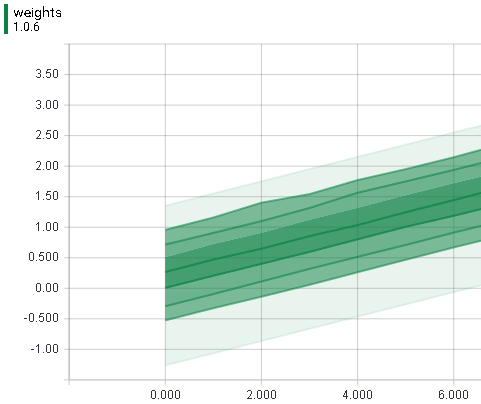
\includegraphics[scale=0.8]{images/Distripution-small.png}
	\caption{Verteilung der Werte in einem Tensor über die Zeit}
	\label{fig:Verteilungsdiagram}
\end{figure}

\noindent
Im Diagramm \ref{fig:Verteilungsdiagram}) wird ein Tensor mit 100 Werten dargestellt. 
Dieser Tensor wurde mit einer Normalverteilung initialisiert, wobei die Standartabweichung bei $0.5$ liegt und der Median zu Beginn bei $0.2$ liegt, mit einer geringen Abweichung. 
Die Linien in diesem Diagramm (\ref{fig:Verteilungsdiagram}) und ihre Einfärbungen präsentieren die Verteilung der Werte im beobachteten Tensor. 
Die Verteilung muss von unten Nach oben gelesen werden, dabei ergibt die unterste Linie den minimal Wert der vorgekommen ist. 
Die nächste Linie besagt, dass 7\% der Werte in dem Bereich zwischen dem geringsten und der zweiten Linie sich befinden, was inklusive des geringsten Wertes ist.  
Der nächste Bereich definiert, wie in einer Normalverteilung, dass bis zu Ende dieses Bereiches 16\% darin befinden. 
Im gesamten sind dies $9$ Markierungen mit 8 Bereichen, welche zusammen alle Werte im Tensor wieder spiegeln. 
Diese Folge an prozentualen Anteilen lauten wie folgend: $min, 7\%, 16\%, 31\%, 50\%, 69\%, 84\%, 93\%, max$. 
Im Diagramm (\ref{fig:VerteilungsdiagrammPython}) ist diese Verteilung besser ersichtlich, zusätzlich befinden sich in der Abbildung \ref{fig:Ergebnistensor} die Rohdaten der Diagramme. 

\begin{figure}
	\centering
	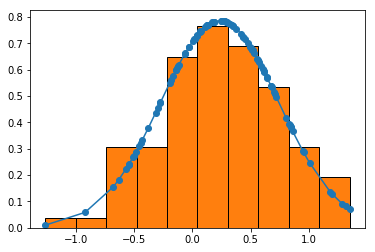
\includegraphics[scale=0.6]{images/gaussian.png}
	\caption{Verteilung der Werte in dem Tensor zu dem Diagramm \ref{fig:Verteilungsdiagram}}
	\label{fig:VerteilungsdiagrammPython}
\end{figure}

\begin{figure}

\lstset{language=Python}
\begin{lstlisting}

 -1.2645409, -0.92252451, -0.68004417, -0.63273954, -0.57005012, 
 -0.5477351, -0.54554129, -0.51146084, -0.50482351, -0.4872272, 
 -0.45631331, -0.44180638, -0.43258488, -0.38066232, -0.31675094, 
 -0.29567719, -0.27768314, -0.27437925, -0.19503899, -0.18343721, 
 -0.16653274, -0.13992153, -0.13946836, -0.12969615, -0.12044857, 
 -0.11908005, -0.06734778, -0.062724337, -0.032598898, -0.02885592, 
 0.006216079, 0.015204117, 0.018379062, 0.036883533, 0.041039094, 
 0.063002124, 0.068820029, 0.072805718, 0.11137276, 0.11735194, 
 0.12555882, 0.12613684, 0.13053563, 0.13633718, 0.17283598, 
 0.18271323, 0.18530971, 0.18671049, 0.24375655, 0.25207496, 
 0.27566099, 0.27588493, 0.27921408, 0.28581429, 0.29526407, 
 0.30613232, 0.32309669, 0.33705187, 0.34577289, 0.34687665, 
 0.37553167, 0.41834235, 0.43759531, 0.4376972, 0.45076531, 
 0.47984695, 0.49715465, 0.50634104, 0.51550949, 0.5168677, 
 0.53031796, 0.5579083, 0.56285316, 0.57165861, 0.59320259, 
 0.60513371, 0.61539149, 0.61814398, 0.63975775, 0.64333171, 
 0.67751783, 0.67795348, 0.68242437, 0.70252627, 0.70793462, 
 0.72128826, 0.80693412, 0.83029318, 0.83635086, 0.84400082, 
 0.84558558, 0.86151552, 0.95068389, 0.95598722, 1.0072051, 
 1.1837469, 1.1992682, 1.285683, 1.3168017, 1.3521272

\end{lstlisting}

	\caption{Sortierter Ergebnistensor zum Verteilungsdiagramm \ref{fig:VerteilungsdiagrammPython} und \ref{fig:Verteilungsdiagram}}
	\label{fig:Ergebnistensor}
\end{figure}


%[maximum, 93%, 84%, 69%, 50%, 31%, 16%, 7%, minimum]
%[maximum, μ+1.5σ, μ+σ, μ+0.5σ, μ, μ-0.5σ, μ-σ, μ-1.5σ, minimum]

%\textbf{TODO Grafik}

\paragraph{Histogram} 
















\chapter{Facial Keypoints Detection}
\label{cha:Facial Keypoints Detection}

\section{Ausgangssituation}

Gesichtserkennung spielt in 21st Jahrhundert eine immer größer werdende Rolle. 
So existieren auch Herausforderungen mit den Schlüsselpunkten im Gesicht eines Menschen, welche wieder für Gesichtserkennungen verwendet werden können. 
Diese Schlüsselpunkte variieren sehr stark von Individuum zu nächsten aber auch jedes Individuum selbst hat eine Menge an Variationen. 
So spielt hier die Größe, die Position, die Neigung sowie die Beleuchtung eine Rolle und erzeugt eine fast unendliche Menge an Möglichkeiten. 
Mit Computer Vision konnten sehr viele Verbesserungen in diesem Bereich erzielt werden, wobei noch sehr viel Raum für Forschung und Verbesserungen bleibt. \newline

\noindent
Die Aufgabenstellung wird auf der Online-Plattform Kaggle \footnote{Kaggle: Facial Keypoints Detection \url{https://www.kaggle.com/c/facial-keypoints-detection}} gehostet wo auch die Trainings- und Testdaten zur Verfügung gestellt werden. 
Diese Aufgabe war im Jahr 2016 eine Herausforderung wo sich jeder beteiligen konnte, um den ersten Platz zu erreichen. 
Das Ziel für jeden Teilnehmer war es ein System zu entwickeln, welches mit den Trainingsdaten trainiert wird.
Im Anschluss sollte dieses System dann mit den Testdaten getestet werden. 
Dieses Ergebnis musste dann eingereicht werden, welches im Anschluss überprüft und bewertet wurde.

\section{Vorbereitung}

Die Daten welche zur Verfügung gestellt werden, sind auf mehreren Dateien aufgeteilt. 
In diesem Fall beinhaltet die Datei mit den Trainingsdaten die meisten Daten. 
Diese Datei beinhaltet die Bilder der Gesichter, sowie die Koordinaten der Schlüsselpunkte, gespeichert in einer CSV-Notation.
Im gesamten Gesicht gibt es 15 Schlüsselpunkte welche hier berücksichtigt werden. 
\begin{figure}[ht!]
\lstset{language=Python}
\begin{lstlisting}
left_eye_center, right_eye_center, 
left_eye_inner_corner, left_eye_outer_corner, right_eyee_inner_corner, right_eye_outer_corner, 
left_eyebrow_inner_end, left_eyebrow_outer_end, right_eyebrow_inner_end, right_eyebrow_outer_end, 
nose_tip, 
mouth_left_corner, mouth_right_corner, 
mouth_center_top_lip, mouth_center_bottom_lip
\end{lstlisting}
	\caption{$15$ Schlüsselpunkte im Gesicht eines Menschen}
	\label{fig:15keypoints}
\end{figure}
Jeder diese Schlüsselpunkte besteht aus einer X und Y Koordinate. 
Diese Datei besitzt zusätzlich in der $31$ Spalte das Bild mit dem dazugehörigen Gesicht.
Das Bild ist Encodiert abgelegt und besteht aus $96 * 96$ Werten. 
In diesem Sinne stehen nur Bilder in Graustufen zur Verfügung mit einer Auflösung von $96 * 96$ Pixel und einer Farbtiefe von $[0, 255]$, wie in der Abbildung \ref{fig:ausgangsdaten} zu erkennen ist. 
Für diese Aufgabe werde im Grunde auch nur die Konturen benötigt, was somit den einen Farbkanal erklärt aber auch die Aufgabe schwieriger macht. 
\begin{figure}
	\centering
	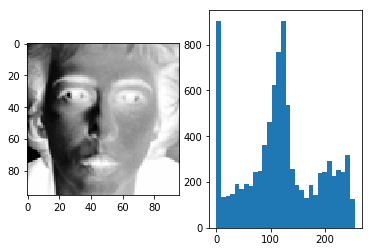
\includegraphics[scale=0.8]{images/ausgangsDaten.png}
	\caption{Ein Gesicht aus dem Datenbestand mit der Verteilung der Graustufenwerten}
	\label{fig:ausgangsdaten}
\end{figure}
\begin{figure}[ht!]
\lstset{language=Python}
	\begin{lstlisting}
# left\_eye\_center, right\_eye\_center
66.0335639098,39.0022736842,30.2270075188,36.4216781955
# left\_eye\_inner\_corner, left\_eye\_outer\_corner
59.582075188,39.6474225564,73.1303458647,39.9699969925
# right\_eye\_inner\_corner, right\_eye\_outer\_corner
36.3565714286,37.3894015038,23.4528721805,37.3894015038
# left\_eyebrow\_inner\_end, left\_eyebrow\_outer\_end
56.9532631579,29.0336481203,80.2271278195,32.2281383459
# right\_eyebrow\_inner\_end, right\_eyebrow\_outer\_end
40.2276090226,29.0023218045,16.3563789474,29.6474706767
# nose\_tip
44.4205714286,57.0668030075
# mouth\_left\_corner, mouth\_right\_corner
61.1953082707,79.9701654135,28.6144962406,77.3889924812
# mouth\_center\_top\_lip, mouth\_center\_bottom\_lip
43.3126015038,72.9354586466,43.1307067669,84.4857744361
# image
238 236 237 238 240 240 239 241 241 243 240 239 231 212 ...
\end{lstlisting}
	\caption{Ein gesamter Datensatz aus den Trainingsdaten mit den X und Y Werten pro Schlüsselpunkt}
	\label{fig:ausgangsdatenRoh}
\end{figure}

\subsection{Daten vorbereiten und normalisieren}

Diese Daten müssen zu Beginn vorbereitet und normalisiert werden. 
Um Problemgröße zu verringern empfiehlt es sich die Aufgabe aufzuteilen auf mehrere Netzwerke. 
Dies hat einen zusätzlichen Grund, da die Trainingsdaten nicht komplett sind und somit nicht zu allen Bildern alle 15 Schlüsselpunkte vorhanden sind. 
Sollte dies ignoriert werden, würde sich die Anzahl der zur Verfügung stehenden Datensätze von $7049$ auf $2140$ reduzieren. 
Ein weiterer Grund für die Auftrennung der Problemstellung ist, da Ressourcen leichter verteilt werden können und die Netzwerke noch fein angepasst werden könnten. \newline

\noindent
Unter der Zuname von Pandas \footnote{Pandas: Python Data Analysis Library \url{http://pandas.pydata.org/}} und NumPy \footnote{NumPy: Scientific Computing \url{http://www.numpy.org/}} besteht die Möglichkeit sehr einfach und Effizient auf die Datensätze zuzugreifen und diese zu Verwenden. 
Wie in der Codebeispiel \ref{fig:datenLesenEinschränken} ersichtlich ist, werden die Daten mit Hilfe von Pandas geladen und unter Zunahme von NumPy normalisiert und neu strukturiert. 
\begin{figure}[ht!]
\lstset{language=Python}
\begin{lstlisting}
import pandas as pd
import numpy as np

# konstanten Definition
IMAGE_SIZE = 96

# Daten einlesen
df = pd.read_csv('~/training.csv')

# Bilder um konvertieren in eine List von Zahlen
df['Image'] = df['Image'].apply(lambda im: np.fromstring(im, sep=' '))

# die Aktuell benötigten Spalten herausnehmen
df = df[['left_eye_center', 'right_eye_center', 'Image']]

# entfernen unvollständiger Datensätze
# Verkleinerung der Datensätze von 7049 auf 7033
df = df.dropna()

# normalisieren der Bilder in einen Wertebereich von [0, 1] 
# und überführen in eine 96 mal 96 Matrix
# Variable X beinhaltet alle Bilder des Datensatzes welche Vollständig sind
X = np.vstack(df['Image']) / 255.
X = X.reshape(-1, IMAGE_SIZE, IMAGE_SIZE, 1)

# explizites definieren des Datentyps für die Werte das Bild
X = X.astype(np.float32)

# normalize the X, Y Koordinaten in einen Wertebereich von [0, 1]
# Variable Y beinhaltet die Labels zu allen Bildern
Y = df[df.columns[:-1]].values
Y = Y / 96.0
\end{lstlisting}
	\caption{Daten einlesen und einschränken}
	\label{fig:datenLesenEinschränken}
\end{figure}

\subsection{Evaluation- und Errorfunktion}

Die Ergebnisse des Netzwerkes müssen in jedem Fall, im Bereich des maschinellen Lernens in der überwachten Form, verglichen und Validiert werden. 
In diesem Beispiel handelt es sich nicht um eine Klassifizierungsaufgabe, sondern um eine Regressionsproblemstellung. 
In diesem Fall kann nicht eine einfach 'Cross Entroy' \textbf{TODO checken} Funktionen verwendet werden, um die Daten zu evaluieren und zu adaptieren. 
Aus diesem Grund muss dies Manuel durchgeführt werden und selbst eine Berechnung aufgestellt werden, welche diese Werte liefert, damit diese einem Optimierer übergeben werden können. 
Der Verlust beziehungsweise die Differenz zwischen Ergebnis des Netzwerkes und dem bekannten Ergebnis, kann durch eine Subtraktion sowie einer Quadrierung berechnet werden. 
Diese ist in der Gleichung \ref{eq:lossCalc} zu erkennen, wobei \textit{graph} eine Matrix (Tensor) an Ergebnissen ist, mit der Anzahl an Zeilen wie in der Konstante \textit{BATCH\_SIZE} definiert. 
Die Variable \textit{train\_labels\_node} beinhaltet die bekannten Ergebnisse zu Bilder mit den selben Dimensionen wie in der Matrix \textit{graph}. 
\textit{tf.subtract} führt eine Subtraktion auf jeden Inhalt der beiden Matrizen aus, was auch dazu führt, dass diese die selben Dimensionen haben müssen. 
\textit{tf.square} quadriert die berechneten Differenzen um negative Werte zu entfernen. 
Zum Abschluss werden alle Ergebnisse in der Ergebnismatrix mit \textit{tf.reduce\_sum} aufsummiert, was zu einem Skalarenergebnis führt. 
Für diese konkrete Implementierung wurde als Opitmierungsalgorithmus ein \textit{Adam}-Algorithmus \textbf{TODO Adam} verwendet. 
Um das Verlustergebnis für einen Leser lesbare zu machen, muss der Verlustwert durch die Anzahl der Batchgröße dividiert werden, was die Differenz in einem Datensatz als Durchschnitt ergibt. 
Die gesamte Umsetzung ist im Codebeispiel \ref{fig:VerlustKonkreOpitimier} zu finden. 
\begin{equation}
	Verlust := \sum{(R - L)^2}
	\label{eq:lossCalc}
\end{equation}
\begin{figure}[ht!]
\lstset{language=Python}
\begin{lstlisting}
import tensorflow as tf

# konstanten Definition
BATCH_SIZE = 64

# Verlustberechnung
with tf.name_scope("loss"):
    # sollte sich im Laufe der Trainingsphasen an 0 annähern
    loss = tf.reduce_sum(
    			tf.square(
    				tf.subtract(graph, train_labels_node)
    			)
    		)

# Auswahl eines konkreten Optimierungsalgorithmuses in der Kurzschreibweise
# mit einer Lernrate von 0.00001
with tf.name_scope("train"):
    train = tf.train.AdamOptimizer(learning_rate=1e-5).minimize(loss)
    
# Verlustwert durch die Anzahl der Bilder im Batch da diese Werte 
# zusammen Summiert werden
with tf.name_scope("accuracy"):    
    accuracy = loss / BATCH_SIZE
\end{lstlisting}
	\caption{Verlustberechnung, konkreter Opitimierungsalgorithmus, Genauigkeitberechnung}
	\label{fig:VerlustKonkreOpitimier}
\end{figure}
 
\section{Neuronale Ebenen vorbereiten}

Damit die Ebenen einfacher verwendet werden können, können dies als konfigurierbare Muster definiert werden. 
Dadurch wird erzielt, dass gleiche Ebenen im visualisierten Graphen die selbe Farbe besitzen und zum anderen alle Inhalte darin zusammengefasst werden. 
Im Grunde existieren zwei verschieden Haupttypen an Ebenen. 
Zum einen die Convolutional-Ebenen und zum anderen die Vollvernetzen-Ebenen. 
Wie im Code \ref{fig:ConvFc} ersichtlich ist besitzen beide Hauptgruppen an Ebenen jeweils eine Datenquelle beschrieben als \textit{x\_} und Gewichtungen und Biaseswerte. 
Die Bias Werte werden dabei immer erst nach der Kernfunktion an das Ergebnis angefügt und somit in der Aktivierungsfunktion berücksichtigt. 
\begin{figure}[ht!]
\lstset{language=Python}
\begin{lstlisting}
def conv_layer(x_, size_in, size_out, name="conv"):
    with tf.name_scope(name):
        weights = tf.Variable(tf.truncated_normal([3, 3, size_in, size_out], dtype=tf.float32, stddev=1e-1), 
                              trainable=True, name='weights')
        conv = tf.nn.conv2d(x_, weights, [1, 1, 1, 1], padding='SAME')
        biases = tf.Variable(tf.constant(0.0, shape=[size_out], dtype=tf.float32), 
                             trainable=True, name='biases')
        bias = tf.nn.bias_add(conv, biases)
        conv = tf.nn.relu(bias, name="act")

    maxPool = tf.nn.max_pool(conv, 
                             ksize=[1, 2, 2, 1],
                             strides=[1, 2, 2, 1],
                             padding='VALID')

    return conv

def fc_layer(x_, size_out, name="fc", act=None):
    with tf.name_scope(name):
        size_in = x_.get_shape()[1].value
        weights = tf.Variable(tf.truncated_normal([size_in, size_out], dtype=tf.float32, stddev=1e-2), 
                              trainable=True, name='weights')
        biases = tf.Variable(tf.constant(0.0, shape=[size_out], dtype=tf.float32), 
                                  trainable=True, name='biases')
        mul = tf.nn.xw_plus_b(x_, weights, biases)
        
        if act is not None:
            mul = act(mul)

        return mul
\end{lstlisting}
	\caption{Definition der Convolutional- und Vollvernetzen-Ebenen}
	\label{fig:ConvFc}
\end{figure}

\section{Neuronale Ebenen verknüpfen}

Diese Definitionen der Ebenen aus dem Codefragment \ref{fig:ConvFc} müssen nun in einem Netzwerk zusammen vernetzt werden. 
Ein neuronales Netzwerk welches relative leichtgewichtig ist und diese Problematik relative brauchbar lösen kann, ist im Grunde ein sehr vereinfachtes 'VGG16' Netzwerk \footcite{VGG16: TODO}.
Für diesen Fall besteht dieses aus $3$ Convolutional-Ebenen und $3$ Vollvernetzen-Ebenen, wie im Codefragment \ref{fig:buildGraph} zu sehen ist. 
Das originale VGG16 Netzwerk besitzt im Gegensatz zu aktuell verwendeten, $5$ Convolutional-Ebenen mit je $2$ integrierten Convolutional-Ebenen mit den selben Dimensionen und die Hauptebenen $3, 4, 5$ sogar $3$ Convolutional-Ebenen. 
Die letzte Ebene der Vollvernetzen-Ebenen wird dabei ohne Aktivierungsfunktion ausgeführt, um die Roh-Ergebnisse zu bekommen. 
Im aktuellen Fall werden für die $2$ Iris-Positionen im Gesicht $4$ Ergebnisse benötigt. 
\begin{figure}[ht!]
\lstset{language=Python}
\begin{lstlisting}
def model(data):
    net = conv_layer(data, 1, 32, "conv1")
    net = conv_layer(net, 32, 64, "conv2")
    net = conv_layer(net, 64, 128, "conv3")

	# Transformieren in eine flache Struktur
    dims = net.get_shape()[1:]
    k = dims.num_elements()
    with tf.name_scope('flatten'):
        net = tf.reshape(net, [-1, k])
    
    net = fc_layer(net, 256, "fc1", tf.nn.relu)    
    net = fc_layer(net, 256, "fc2", tf.nn.relu)
    net = fc_layer(net, 4, "fc3")
    
    return net
    
# Definition der Platzhalter für die Datenübergabe
train_data_node = tf.placeholder(tf.float32, shape=(BATCH_SIZE, IMAGE_SIZE, IMAGE_SIZE, 1))
train_labels_node = tf.placeholder(tf.float32, shape=(BATCH_SIZE, 4))

# erstellen eines Graphen mit dem definierten Model
graph = model(train_data_node)
\end{lstlisting}
	\caption{Modeldefinition des Graphen}
	\label{fig:buildGraph}
\end{figure}

\section{Trainieren}

Um das erzeugte Netzwerk aus \ref{fig:buildGraph} verwenden und trainieren zu können, muss dieses zu erst Initialisiert werden. 
Wie im Code \ref{fig:initRun} zu erkennen ist wird ein globale Initialisierung verwendet welchen alle Konstanten und Variablen der aktuellen Umgebung initialisiert. 
In der For-Schleife werden fast alle Datensätze einmal durch den Graphen gesendet und entweder zum Trainieren oder Evaluieren verarbeitet. 
Der Session wird in der \textit{Run}-Methode eine Liste and Endpunkten des Graphen mitgegeben welche Evaluiert werden sollen. 
In der Trainingsphase ist dies der Optimierungsendpunkt und in der Evaluierungsphase die Punkte \textit{accuracy} und \textit{graph}. 
Accuracy damit ein vergleichbarer Wert zur Verfügung steht, an welchem der Lernfortschritt erkennbar ist und der Hauptendpunkt des Graphen selbst, damit die Ergebnis direkt in die Bilder gezeichnet werden können. 
Dies ermöglicht eine visualisierte Verifikation durch einen Supervisor. 
\begin{figure}[ht!]
\lstset{language=Python}
\begin{lstlisting}
# erstellen einer Session
sess = tf.Session()

# erstellen einer globalen Initialisierungsroutine
init_op = tf.global_variables_initializer()
# initialisieren aller Konstanten und Variablen
sess.run(init_op)

# durchlaufen aller Datensätze
runing = train_data.shape[0] // BATCH_SIZE
for i in range(runing):
    offset = i * BATCH_SIZE
    
    # laden eines Datenbatches aus den Datensätzen
    batch_data = train_data[offset:(offset + BATCH_SIZE), ...]
    batch_labels = train_labels[offset:(offset + BATCH_SIZE)]
    
    # ersetzen der Platzhalter durch die konkreten Daten
    feed = {train_data_node: batch_data, 
            train_labels_node: batch_labels}
     
    # ausführen des Graphen zur Evaluierung
    if i % 5 == 0:
        [train_accuracy, data] = sess.run([accuracy, graph], feed_dict=feed)
        print data[0:4]
        print batch_labels[0:4]
        
        print i, train_accuracy
        
    # ausführen einer Trainingsiteration
    else:
        sess.run(train, feed_dict=feed)
\end{lstlisting}
	\caption{Initialisierung des Graphen und durchführen einer Epoche}
	\label{fig:initRun}
\end{figure}

\section{Validierungsresultate}







%\include{Zusammenfassung_Ausblick} % Stephan TODO
%\include{diplomschrift}
%\include{latex}
%\include{abbildungen}
%\include{mathematik}
%\chapter[Umgang mit Literatur]{Umgang mit Literatur und anderen Quellen}
\label{cha:Literatur}

\paragraph{Anmerkung:}
Der Titel dieses Kapitels ist absichtlich so
lang geraten, dass er nicht mehr in die Kopfzeile der Seiten passt. 
In diesem Fall kann in der \verb!\chapter!-Anweisung 
als optionales Argument \verb![..]! ein verkürzter Text für die
Kopfzeile (und das Inhaltsverzeichnis) angegeben werden:
%
\begin{LaTeXCode}[numbers=none]
\chapter[Umgang mit Literatur]{Umgang mit Literatur und anderen Quellen}
\end{LaTeXCode}

\section{Allgemeines}

Der richtige Umgang mit Quellen ist ein wesentliches Element bei der Erstellung
wissenschaftlicher Arbeiten im Allgemeinen (\sa\ Abschnitt \ref{sec:Plagiarismus}).
Für die Gestaltung von Quellenangaben sind unterschiedlichste Richtlinien in
Gebrauch, bestimmt \ua\ vom jeweiligen Fachgebiet oder Richtlinien von Verlagen und Hochschulen.
Diese Vorlage sieht ein Schema vor, das in den natur\-wissen\-schaftlich-technischen 
Disziplinen üblich ist.%
\footnote{Anpassungen an andere Formen sind relativ leicht möglich.}
Technisch basiert dieser Teil auf \texttt{BibTeX} \cite{Patashnik88}
\bzw\ \texttt{Biber}%
\footnote{Wird seit Version 2013/02/19 anstelle von \texttt{bibtex} verwendet 
	(s.\ \url{http://biblatex-biber.sourceforge.net/}),}
in Kombination mit dem Paket \texttt{biblatex} \cite{Lehman2014}.


Die Verwaltung von Quellen besteht grundsätzlich aus zwei Elementen: 
\emph{Quellenverweise} im Text beziehen sich auf Einträge im \emph{Quellenverzeichnis}
(oder in mehreren Quellenverzeichnissen).
Das Quellenverzeichnis ist eine
Zusammenstellung aller verwendeten Quellen, typischerweise ganz am Ende des Dokuments.
Wichtig ist, dass jeder Quellenverweis einen zugehörigen, eindeutigen
Eintrag im Quellenverzeichnis aufweist und jedes Element im Quellenverzeichnis auch
im Text referenziert wird.



\section{Quellenverweise}

Um einen Eintrag im Quellenverzeichnis zu erstellen und im Text darauf zu verweisen, stellt \latex ein zentrales Kommando zur Verfügung.

\subsection{Das {\tt {\bs}cite} Makro}

Für Quellenverweise im laufenden Text verwendet man die Anweisung
\begin{itemize}
\item[] \verb!\cite{!\textit{Verweise}\verb!}! 
				\quad oder \quad
        \verb!\cite[!\textit{Zusatztext}\verb!]{!\textit{Verweise}\verb!}!.
\end{itemize}

\noindent%
\textit{Verweise} ist eine durch Kommas getrennte Auflistung von $1$--$n$ Quellen-\emph{Schlüsseln}
zur Identifikation der entsprechenden Einträge im Quellenverzeichnis.
Mit \textit{Zusatztext} können Ergänzungstexte zum aktuellen Quellenverweis angegeben
werden, wie \zB Kapitel- oder Seitenangaben bei Büchern.
Einige Beispiele dazu:
\begin{itemize}
\item[] \verb!Mehr dazu findet sich in \cite{Kopka2003}.! \newline
      $\rightarrow$ Mehr dazu findet sich in \cite{Kopka2003}.
\item[] \verb!Mehr über \emph{Styles} in \cite[Kap.\ 3]{Kopka2003}.! \newline
      $\rightarrow$ Mehr über \emph{Styles} in \cite[Kap.\ 3]{Kopka2003}.
\item[] \verb!Die Angaben in \cite[S.\ 274--277]{Ears99} sind falsch.! \newline
      $\rightarrow$ Die Angaben in \cite[S.\ 274--277]{Ears99} sind aus meiner Sicht falsch.
\item[] \verb!Überholt sind auch \cite{Ears99,Patashnik88,Duden97}.! \newline
      $\rightarrow$ Überholt sind auch \cite{Ears99,Patashnik88,Duden97}.
\end{itemize}
Die Sortierung der Angaben im letzten Beispiel erfolgt automatisch.



\subsection{Häufige Fehler}

\subsubsection{Verweise außerhalb des Satzes}
Quellenverweise sollten innerhalb oder am Ende eines Satzes (\dah vor
dem Punkt) stehen, nicht \emph{außerhalb}:
%
\begin{center}
\begin{tabular}{rl}
 \textbf{Falsch:}  & \ldots hier ist der Satz aus. \cite{Oetiker2014} Und jetzt geht es weiter \ldots \\
 \textbf{Richtig:} & \ldots hier ist der Satz aus \cite{Oetiker2014}. Und jetzt geht es weiter \ldots
\end{tabular}
\end{center}

\subsubsection{Zitate}
Falls ein ganzer Absatz (oder mehr) aus einer Quelle zitiert wird,
sollte der Verweis im vorlaufenden Text und nicht
\emph{innerhalb} des Zitats selbst platziert werden. Als Beispiel die folgende Passage
aus \cite{Oetiker2014}:
\begin{quote}
Typographical design is a craft. Unskilled authors often commit
serious formatting errors by assuming that book design is mostly a
question of aesthetics---``If a document looks good artistically,
it is well designed.'' But as a document has to be read and not
hung up in a picture gallery, the readability and
understandability is of much greater importance than the beautiful
look of it.%
\footnote{Man beachte die Verwendung von englischen Hochkommas innerhalb dieses
Zitats.}
\end{quote}
Für das Zitat selbst sollte übrigens die dafür vorgesehene Umgebung
%
\begin{itemize}
 \item[] \verb!\begin{quote}! \emph{Zitierter Text ...} \verb!\end{quote}!
\end{itemize}
%
verwendet werden, die durch beidseitige Einrückungen das
Zitat vom eigenen Text klar abgrenzt und damit die Gefahr von
Unklarheiten (wo ist das Ende des Zitats?) mindert.
Wenn gewünscht, kann das Innere des Zitats auch in Hochkommas verpackt 
\emph{oder} kursiv gesetzt werden -- aber nicht beides!



\subsection{Umgang mit Sekundärquellen}

In seltenen Fällen kommt es vor, dass man eine Quelle \textbf{A} angeben
möchte (oder muss), die man zwar nicht zur Hand -- und damit auch nicht selbst gelesen --
hat, die aber in einer \emph{anderen}, vorliegenden Quelle \textbf{B} zitiert wird.
In diesem Fall wird \textbf{A} als \emph{Original-} oder \emph{Primärquelle} und \textbf{B} 
als \emph{Sekundärquelle} bezeichnet. Dabei sollten folgende Grundregeln beachtet werden:
%
\begin{itemize}
\item
\textbf{Sekundärquellen} nach Möglichkeit überhaupt \textbf{vermeiden}!
\item
Um eine Quelle in der üblichen Form zitieren zu können, muss man sie \textbf{immer selbst
eingesehen} (gelesen) haben!
\item
Nur wenn man die Quelle wirklich \textbf{nicht} beschaffen kann, ist ein Verweis über eine Sekundärquelle
zulässig. In diesem Fall sollten korrekterweise Pri\-mär- und Sekundärquelle \emph{gemeinsam} 
angegeben werden, wie im nachfolgenden Beispiel gezeigt.
\item
\textbf{Wichtig:} In das Quellenverzeichnis wird \textbf{nur die tatsächlich vorliegende Quelle} 
(\textbf{B}) und nicht die Originalarbeit aufgenommen!
\end{itemize}
%
\textbf{Beispiel:} Angenommen man möchte aus dem berühmten Buch \emph{Dialogo} von Galileo Galilei 
(an das man nur schwer herankommt) eine Stelle zitieren, die man in einem neueren Werk aus dem Jahr 1969 
gefunden hat. Das könnte man \zB\ mit folgender Fußnote bewerkstelligen.%
\footnote{Galileo Galilei, \emph{Dialogo sopra i due massimi sistemi del mondo tolemaico e copernicano}, 
S.~314 (1632). Zitiert nach \cite[S.~59]{Hemleben1969}.} % Alle Seitennummern sind frei erfunden!


\section{Quellenverzeichnis}

Für die Erstellung des Quellenverzeichnisses gibt es in \latex zwei
Möglichkeiten:
\begin{enumerate}
\item Das Quellenverzeichnis manuell zu formatieren (nicht zu empfehlen, 
s.\ \cite[Abschn.\ 11.3]{Kopka2003}).
\item Die Verwendung von \texttt{BibTeX}/\texttt{Biber} und einer zugehörigen 
"`Literaturdatenbank"' (s.\ \cite[Kap.\ 12]{Kopka2003}).
\end{enumerate}
Tatsächlich ist die erste Variante nur bei sehr wenigen Literaturangaben interessant.
Die Arbeit mit \texttt{BibTeX}/\texttt{biber} macht sich hingegen schnell bezahlt und ist zudem wesentlich
flexibler.

\subsection{Literaturdaten in BibTeX}
\label{sec:bibtex}

BibTeX ist ein eigenständiges Programm, das aus einer "`Literaturdatenbank"' (eine oder mehrere
Textdateien mit vorgegebener Struktur) ein für \latex geeignetes Quellenverzeichnis
erzeugt. Literatur zur Verwendung von BibTeX findet sich online, \zB \cite{Feder2006,Patashnik88}.
Die BibTeX-Datei zu dieser Vorlage ist \nolinkurl{literatur.bib} (im Hauptverzeichnis).

BibTeX-Dateien können natürlich mit einem Texteditor manuell erstellt werden und für
viele Literaturquellen sind bereits fertige BibTeX-Einträge online verfügbar.
Dabei sollte man allerdings vorsichtig sein, denn diese Einträge sind (auch bei großen
Institutionen und Verlagen) \textbf{häufig falsch oder syntaktisch fehlerhaft}!
Man sollte sie daher nicht ungeprüft übernehmen und insbesondere die Endergebnisse genau kontrollieren.
Darüber hinaus gibt es eigene Anwendungen zur Wartung von
BibTeX-Verzeichnissen, wie beispielsweise
\emph{JabRef}.\footnote{\url{http://jabref.sourceforge.net/}}


\subsubsection{Verwendung von \texttt{biblatex} und \texttt{biber}}

Dieses Dokument verwendet \texttt{biblatex} (Version 1.4 oder höher) in Verbindung
mit dem Programm \texttt{biber}, 
das viele Unzulänglichkeiten des traditionellen BibTeX-Work\-flows behebt und dessen Möglichkeiten deutlich erweitert.%
\footnote{Tatsächlich ist \texttt{biblatex} die erste radikale (und längst notwendige) Überarbeitung des mittlerweile stark in die Jahre gekommenen BibTeX-Workflows. Zwar wird dabei BibTex weiterhin für 
die Sortierung der Quellen verwendet, die Formatierung der Einträge und viele andere Elemente werden jedoch ausschließlich über \latex-Makros gesteuert.}
Allerdings sind die in \texttt{biblatex} verwendeten Literaturdaten nicht mehr vollständig 
rückwärts-kompatibel zu BibTeX. Es ist daher in der Regel notwendig, bestehende oder aus
Online-Quellen übernommene BibTeX-Daten manuell zu überarbeiten (\sa\ Abschnitt~\ref{sec:TippsZuBibtex}).

In dieser Vorlage sind die Schnittstellen zu \texttt{biblatex} weitgehend in der Datei \nolinkurl{hgbthesis.cls} verpackt. Die typische Verwendung in der \latex-Haupt\-datei sieht folgendermaßen aus:
%
\begin{LaTeXCode}[numbers=none]
\documentclass[master,german]{hgbthesis}
   ...
\bibliography{literatur} /+\label{tex:literatur1}+/
   ...
\begin{document}
   ...
\MakeBibliography{Quellenverzeichnis} /+\label{tex:literatur2}+/
\end{document}
\end{LaTeXCode}
%
In der "`Präambel"' (Zeile \ref{tex:literatur1}) wird mit \verb!\bibliography{literatur}! 
auf eine (modifizierte) BibTex-Datei \nolinkurl{literatur.bib} verwiesen.%
\footnote{Das Makro 
\texttt{{\bs}bibliography} ist eigentlich ein Relikt aus BibTeX
und wird in \texttt{biblatex} durch die Anweisung \texttt{{\bs}addbibresource} 
ersetzt. Beide Anweisungen sind gleichwertig, allerdings wird nur mit 
\texttt{{\bs}bibliography} die zugehörige \texttt{.bib}-Datei im Fileverzeichnis von TeXnicCenter angezeigt.}
Falls mehrere BibTeX-Dateien verwendet werden, können sie in der gleichen Form angegeben werden.

Die Anweisung \verb!\MakeBibliography{..}! am Ende des Dokuments (Zeile~\ref{tex:literatur2})
besorgt die Ausgabe des Quellenverzeichnisses, hier mit dem Titel "`Quellenverzeichnis"'.
Dabei sind zwei Varianten möglich:
%
\begin{description}
\item[\texttt{{\bs}MakeBibliography\{title\}}] ~ \newline
   Erzeugt ein in mehrere \emph{Kategorien} (s.\ Abschnitt \ref{sec:BibKategorien}) geteiltes Quellenverzeichnis 
   mit der Hauptüberschrift \texttt{title}. Diese Variante wird im vorliegenden Dokument verwendet.
\item[\texttt{{\bs}MakeBibliography[nosplit]\{title\}}] ~ \newline
   Erzeugt ein traditionelles \emph{einteiliges} Quellenverzeichnis mit der
   Überschrift \texttt{title}. 
\end{description}
%
Die Überschrift \texttt{title} scheint in beiden Fällen ohne Nummerierung 
im Inhaltsverzeichnis auf (auf \texttt{chapter}-Ebene).
Bei geteiltem Quellenverzeichnis werden die Überschriften der einzelnen Abschnitte auf 
\texttt{section}-Ebene eingetragen.


\subsection{Kategorien von Quellenangaben}
\label{sec:BibKategorien}

Für geteilte Quellenverzeichnisse sind in dieser Vorlage folgende drei Kategorien vorgesehen
(s.\ Tabelle \ref{tab:QuellenUndEintragstypen}):%
\footnote{Diese sind in der Datei \nolinkurl{hgbthesis.cls} definiert.
Allfällige Änderungen sowie die Definition zusätzlicher Kategorien sind 
bei Bedarf relativ leicht möglich.}
%
\begin{description}
	\item[\texttt{literature}] -- für alle Quellen, die in gedruckter Form vorliegen;
	\item[\texttt{avmedia}] -- für Filme, audio-visuelle Medien und Computer Games (auf DVD, CD, \usw);
	\item[\texttt{online}] -- für Werke, die \emph{ausschließlich} online verfügbar sind.
\end{description}
%
Jedes Quellenobjekt wird aufgrund des angegebenen BibTeX-Eintragtyps 
\texttt{@\emph{type}} automatisch einer dieser Kategorien 
zugeordnet (s.\ Tabelle~\ref{tab:BibKategorien}).
Angeführt sind hier nur die wichtigsten Eintragstypen, die allerdings die meisten
Fälle in der Praxis abdecken sollten und nachfolgend durch Beispiele erläutert sind.
Alle nicht explizit angegebenen Einträge werden grundsätzlich in der Kategorie \emph{literature} 
ausgegeben.

\begin{table}
\caption{Quellenarten und empfohlene BibTeX-Eintragstypen.}
\label{tab:QuellenUndEintragstypen}
\centering
\begin{tabular}{llc}
	\hline
	Kategorie \emph{literature} & \texttt{@\emph{type}} & Seite\\
	\hline
	Buch (Textbuch, Monographie) & \texttt{@book} & \pageref{sec:@book}\\
	Sammelband (Hrsg.\ + mehrere Autoren) & \texttt{@incollection} & \pageref{sec:@incollection} \\
	Konferenz-, Tagungsband & \texttt{@inproceedings} & \pageref{sec:@inproceedings}\\
	Beitrag in Zeitschrift, Journal & \texttt{@article} & \pageref{sec:@article}\\
	Bachelor-, Master-, Diplomarbeit, Dissertation & \texttt{@thesis} & \pageref{sec:@thesis}\\
	Technischer Bericht, Laborbericht & \texttt{@techreport} & \pageref{sec:@techreport}\\
	Handbuch, Produktbeschreibung, Norm & \texttt{@manual} & \pageref{sec:@manual}\\
	Gesetzestext, Verordnung etc. & \texttt{@misc} & \pageref{sec:@misc}\\
%
	\hline
	Kategorie \emph{avmedia} & \\
	\hline
	Audio (CD) & \texttt{@audio} & \pageref{sec:@audio}\\
	Video (auf VHS, DVD, Blu-ray Disk) & \texttt{@video} & \pageref{sec:@video}\\
	Film (Kino) & \texttt{@movie} & \pageref{sec:@movie}\\
	Computer Game, Softwareprodukt & \texttt{@software} & \pageref{sec:@software}\\
%
	\hline
	Kategorie \emph{online} & \\
	\hline
	Webseite, Wiki-Eintrag, Blog etc. & \texttt{@online} & \pageref{sec:@online-www}\\
	Online-Video, Bild, Grafik & \texttt{@online} & \pageref{sec:@online-video}\\
\end{tabular}
\end{table}


\begin{table}
\caption{Kategorien von Quellenangaben und zugehörige BibTeX-Eintragstypen.
Bei geteiltem Quellenverzeichnis werden die Einträge jeder Kategorie in einem
eigenen Abschnitt gesammelt.
Grau gekennzeichnete Elemente sind Synonyme für die jeweils darüber stehenden Typen.}
\label{tab:BibKategorien}
\centering
\definecolor{midgray}{gray}{0.5}
\setlength{\tabcolsep}{6mm}
\begin{tabular}{lll}
	\emph{literature} & \emph{avmedia} & \emph{online} \\
	\hline
	\texttt{@book}          & \texttt{@audio}                & \texttt{@online} \\
	\texttt{@incollection}  & \texttt{\color{midgray}@music} & \texttt{\color{midgray}@electronic} \\
	\texttt{@inproceedings} & \texttt{@video}                & \texttt{\color{midgray}@www} \\
	\texttt{@article}       & \texttt{@movie}                &  \\
	\texttt{@thesis}        & \texttt{@software}             &  \\
	\texttt{@techreport}    &  &  \\
	\texttt{@manual}        &  &  \\
	\texttt{@misc}          &  &  \\
	\ldots                  &  &  \\
	\hline
\end{tabular}
\end{table}

%%------------------------------------------------------

\subsection{Gedruckte Quellen (\emph{literature})}
\label{sec:KategorieLiterature}

Diese Kategorie umfasst alle Werke, die in gedruckter Form publiziert wurden,
also beispielsweise in Büchern, Konferenzbänden, Zeitschriftenartikeln, Diplomarbeiten \usw
In den folgenden Beispielen ist jeweils der BibTeX-Eintrag in der Datei \nolinkurl{literatur.bib}
angegeben, gefolgt vom zugehörigen Ergebnis im Quellenverzeichnis.


\subsubsection{\texttt{@book}}
\label{sec:@book}
Ein einbändiges Buch (Monographie), das von einem Autor oder mehreren Autoren zur Gänze gemeinsam verfasst und (typischerweise) von einem Verlag herausgegeben wurde.
% 
\begin{itemize}
\item[] 
\begin{GenericCode}[numbers=none]
@book{BurgerBurge06,
    author={Burger, Wilhelm and Burge, Mark},
    title={Digitale Bildverarbeitung},
	  subtitle={Eine Einführung mit Java und ImageJ},
    publisher={Springer-Verlag},
    location={Heidelberg},
    edition={2},
    year={2005},
    hyphenation={german}
}
\end{GenericCode}
\item[\cite{BurgerBurge06}]
Wilhelm Burger und Mark Burge. \textit{Digitale Bildverarbeitung. Eine
Einführung mit Java und ImageJ}. 2.\ Aufl.\ Heidelberg: Springer-Verlag,
2006.
\end{itemize}
%\printbibliography[keyword=bookexample1,heading=noheader]\nocite{BurgerBurge06}
%
\emph{Hinweis:} Die Auflagennummer (\texttt{edition}) wird üblicherweise nur angegeben, 
wenn es \emph{mehr} als eine Ausgabe gibt -- also insbesondere \textbf{nicht für die 1.\ Auflage}, 
wenn diese die einzige ist!
\textbf{ISBN-Nummern} sollte man auch getrost \textbf{weglassen}.

%%------------------------------------------------------

\subsubsection{\texttt{@incollection}}
\label{sec:@incollection}
Ein in sich abgeschlossener und mit einem eigenen Titel versehener
Beitrag eines oder mehrerer Autoren in einem Buch oder Sammelband.
Dabei ist \texttt{title} der Titel des Beitrags, \texttt{booktitle} der Titel des Sammelbands und
\texttt{editor} der Name des Herausgebers.
%
\begin{itemize}
\item[] 
\begin{GenericCode}[numbers=none]
@incollection{Ears99,
  author={Burge, Mark and Burger, Wilhelm},
  title={Ear Biometrics},
  booktitle={Biometrics: Personal Identification in Networked Society},
  publisher={Kluwer Academic Publishers},
  year={1999},
  location={Boston},
  editor={Jain, Anil K. and Bolle, Ruud and Pankanti, Sharath},
  chapter={13},
  pages={273-285},
  hyphenation={english}
}
\end{GenericCode}
\item[\cite{Ears99}]
Mark Burge und Wilhelm Burger. "`Ear Biometrics"'. In:\ \textit{Biometrics:
Personal Identification in Networked Society}. Hrsg.\ von Anil K.\ Jain,
Bolle Ruud und Pankanti Sharath. Boston:\ Kluwer Academic Publis-
hers, 1999. Kap.\ 13, S.\ 273--285.
\end{itemize}
%\printbibliography[keyword=incollectionexample1,heading=noheader]\nocite{Ears99}

%%------------------------------------------------------

\subsubsection{\texttt{@inproceedings}}
\label{sec:@inproceedings}
Konferenzbeitrag, individueller Beitrag in einem Tagungsband.
Man beachte die Verwendung des neuen Felds \texttt{venue}
zur Angabe des Tagungsorts und 
\texttt{location} für den Ort der Publikation (des Verlags).

\begin{itemize}
\item[]
\begin{GenericCode}[numbers=none]
@inproceedings{Burger87,
	author={Burger, Wilhelm and Bhanu, Bir},
	title={Qualitative Motion Understanding},
	booktitle={Proceedings of the Intl.\ Joint Conference on Artificial Intelligence},
	year={1987},
	month={5},
	editor={McDermott, John P.},
	venue={Mailand},
	publisher={Morgan Kaufmann Publishers},
	location={San Francisco},
	pages={819-821},
	hyphenation={english}
}
\end{GenericCode}
\item[\cite{Burger87}]
Wilhelm Burger und Bir Bhanu. "`Qualitative Motion Understanding"'.
In:\ \textit{Proceedings of the Intl.\ Joint Conference on Artificial Intelligence}.
(Mailand). Hrsg.\ von John P.\ McDermott. San Francisco:\ Morgan
Kaufmann Publishers, Mai 1987, S.\ 819--821.
\end{itemize}
%\printbibliography[keyword=inproceedingsexample1,heading=noheader]\nocite{Burger87}

%%------------------------------------------------------

\subsubsection{\texttt{@article}}
\label{sec:@article}
Beitrag in einer Zeitschrift, einem wissenschaftlichen Journal oder einer Tageszeitung.
Dabei steht \texttt{volume} üblicherweise für den Jahrgang und \texttt{number} für die 
Nummer innerhalb des Jahrgangs. Der Zeitschriftennamen (\texttt{journal} oder
\texttt{journaltitle}) sollte nur in begründeten Fällen abgekürzt werden, um Missverständnisse
zu vermeiden.
%
\begin{itemize}
\item[]
\begin{GenericCode}[numbers=none]
@article{Mermin89,
	author={Mermin, Nathaniel David},
	title={What's wrong with these equations?},
	journal={Physics Today},
	volume={42},
	number={10},
	year={1989},
	pages={9-11},
	hyphenation={english}
}
\end{GenericCode}
\item[\cite{Mermin89}]
Nathaniel David Mermin. "`What's wrong with these equations?"' In:\ \textit{Physics
Today} 42.10 (1989), S. 9--11.
\end{itemize}
%\printbibliography[keyword=articleexample1,heading=noheader]\nocite{Mermin89}
%
\emph{Hinweis:} Die Angabe einer Ausgabe für \emph{mehrere} Monate ist in \texttt{biblatex} nicht mehr
über das Feld \texttt{month} möglich, denn dieses darf nur mehr \emph{einen} Wert enthalten.
In diesem Fall kann jedoch einfach das \texttt{issue}-Feld verwendet (\zB\ \verb!issue={Mai/Juni}!
im BibTeX-Eintrag zu \cite{Guttman01}) und das \texttt{number}-Feld weggelassen werden.


%%------------------------------------------------------

\subsubsection{\texttt{@thesis}}
\label{sec:@thesis}
Dieser (neue) Eintragstyp kann allgemein für akademische Abschlussarbeiten verwendet werden. Er ersetzt
insbesondere die bekannten BibTeX-Einträge \texttt{@phdthesis} (für Dissertationen) sowie
\texttt{@mastersthesis} (für Di\-plom- und Masterarbeiten), die allerdings weiterhin verwendet werden können. Zusätzlich ist damit etwa auch die Angabe von Bachelorarbeiten möglich.

\bigskip % kludge to force heading to next page
\paragraph{Dissertation (Doktorarbeit):}
\begin{itemize}
\item[]
\begin{GenericCode}[numbers=none]
@thesis{Eberl87,
	author={Eberl, Gerhard},
	title={Automatischer Landeanflug durch Rechnersehen},
	type={phdthesis},
	year={1987},
	month={8},
	institution={Universität der Bundeswehr, Fakultät für Raum- und Luftfahrttechnik},
	location={München},
	hyphenation={german}
}
\end{GenericCode}
\item[\cite{Eberl87}]
Gerhard Eberl. "`Automatischer Landeanflug durch Rechnersehen"'.
Diss.\ München:\ Universität der Bundeswehr, Fakultät für Raum- und
Luftfahrttechnik, Aug.\ 1987.
\end{itemize}
%\printbibliography[keyword=phdthesisexample1,heading=noheader]\nocite{Eberl87}

\paragraph{Magister- oder Masterarbeit:} ~ \newline
Analog zur Dissertation (s.\ oben), allerdings mit \texttt{type=\{mathesis\}}.%
%\footnote{Man beachte dabei, dass offiziell (zumindest in Österreich) auch die 
%Abschlussarbeiten von \emph{Master}studiengängen weiterhin als "`Diplomarbeiten"' 
%bezeichnet werden.} % ab März 2012 gilt das nicht mehr

%%------------------------------------------------------

\paragraph{Diplomarbeit:} ~ \newline
Analog zur Dissertation (s.\ oben), allerdings mit \texttt{type=\obnh\{Diplomarbeit\}}:%
%
\begin{itemize}
\item[]
\begin{GenericCode}[numbers=none]
@thesis{Artner07,
	author={Artner, Nicole Maria},
	title={Analyse und Reimplementierung des Mean-Shift Tracking-Verfahrens},
	type={Diplomarbeit},
	year={2007},
	month={7},
	institution={University of Applied Sciences Upper Austria, Digitale Medien},
	location={Hagenberg, Austria},
	url={http://theses.fh-hagenberg.at/thesis/Artner07},
  hyphenation={german}
}
\end{GenericCode}
\item[\cite{Artner07}]
Nicole Maria Artner. "`Analyse und Reimplementierung des Mean-Shift
Tracking-Verfahrens"'. Diplomarbeit. Hagenberg, Austria:\ Upper 
Austria University of Applied Sciences, Digitale Medien, Juli 2007. 
\textsc{url}:\ \url{http://theses.fh-hagenberg.at/thesis/Artner07}.
\end{itemize}
%\printbibliography[keyword=diplomarbeitexample1,heading=noheader]\nocite{Artner07}
%
Der Inhalt des Felds \verb!url={..}! wird dabei automatisch und ohne zusätzliche
Kennzeichnung als URL gesetzt (mit dem \verb!\url{..}! Makro).

%%------------------------------------------------------

\paragraph{Bachelorarbeit:} ~ \newline
Bachelorarbeiten gelten in der Regel zwar nicht als "`richtige"' Publikationen, bei Bedarf müssen sie aber dennoch referenziert werden können. 
%
\begin{itemize}
\item[]
\begin{GenericCode}[numbers=none]
@thesis{Bacher04,
	author={Bacher, Florian},
	title={Interaktionsmöglichkeiten mit Bildschirmen und großflächigen Projektionen},
	type={Bachelorarbeit},
	year={2004},
	month={6},
	institution={Upper Austria University of Applied Sciences, Medientechnik und {-design}},
	location={Hagenberg, Austria},
	hyphenation={german},
	keywords={bachelorarbeitexample1} 
}
\end{GenericCode}
\item[\cite{Bacher04}]
Florian Bacher. "`Interaktionsmöglichkeiten mit Bildschirmen und groß-
flächigen Projektionen"'. Bachelorarbeit. Hagenberg, Austria:\ Upper
Austria University of Applied Sciences, Medientechnik und {-design},
Juni 2004.
\end{itemize}
%\printbibliography[keyword=bachelorarbeitexample1,heading=noheader]\nocite{Bacher04}
%


%%------------------------------------------------------

\subsubsection{\texttt{@techreport}}
\label{sec:@techreport}
Das sind typischerweise nummerierte Berichte (\emph{technical reports}) aus Unternehmen, 
Hochschulinstituten oder Forschungsprojekten.
Wichtig ist, dass die herausgebende Organisationseinheit (Firma, Institut, Fakultät \etc) und 
Adresse angegeben wird. Sinnvollerweise wird auch der zugehörige URL angegeben, sofern vorhanden. 
%
\begin{itemize}
\item[]
\begin{GenericCode}[numbers=none]
@techreport{Drake48,
  author={Drake, Huber M. and McLaughlin, Milton D. and Goodman, Harold R.},
  title={Results obtained during accelerated transonic tests of the {Bell} {XS-1} airplane in flights to a {MACH} number of 0.92},
  institution={NASA Dryden Flight Research Center},
  year={1948},
  month={1},
  location={Edwards, CA},
  number={NACA-RM-L8A05A},
  url={http://www.nasa.gov/centers/dryden/pdf/...05A.pdf},
  hyphenation={english}
}
\end{GenericCode}
\item[\cite{Drake48}]
Huber M.\ Drake, Milton D.\ McLaughlin und Harold R.\ Goodman.
\textit{Results obtained during accelerated transonic tests of the Bell XS-1
airplane in flights to a MACH number of 0.92}. Techn.\ Ber.\ NACA-
RM-L8A05A. Edwards, CA:\ NASA Dryden Flight Research Center,
Jan. 1948. \textsc{url}:\ \url{http://www.nasa.gov/centers/dryden/pdf/87528main_RM-L8A05A.pdf}.
\end{itemize}
%\printbibliography[keyword=techreportexample1,heading=noheader]\nocite{Drake48}

%%------------------------------------------------------

\subsubsection{\texttt{@manual}}
\label{sec:@manual}
Dieser Publikationstyp bietet sich für Dokumente an, bei denen üblicherweise kein Autor genannt ist, wie etwa bei Produktbeschreibungen von Herstellern, Anleitungen, Präsentationen, Normen, White Papers \usw
%
\begin{itemize}
\item[]
\begin{GenericCode}[numbers=none]
@manual{amsldoc02,
	author={{American Mathematical Society}},
	title={User's Guide for the {\tt amsmath} Package},
	year={2002},
	month={2},
	version={2.0},
	url={ftp://ftp.ams.org/pub/tex/doc/amsmath/amsldoc.pdf},
	hyphenation={english}
}
\end{GenericCode}
\item[\cite{amsldoc02}]
American Mathematical Society. 
\textit{User's Guide for the {\tt amsmath} Package}. 
Version 2.0. Feb. 2002. \textsc{url}: \url{ftp://ftp.ams.org/pub/tex/doc/amsmath/amsldoc.pdf}.
\end{itemize}
%\printbibliography[keyword=manualexample1,heading=noheader]\nocite{amsldoc02}
%
In obigem Beispiel gilt zu beachten: 
Da kein Autor bekannt ist, wird hier der Name des \emph{Unternehmens} oder der \emph{Institution} im \texttt{author}-Feld angegeben, allerdings innerhalb einer \textbf{zusätzlichen Klammer} \texttt{\{..\}}, damit das Argument nicht fälschlicherweise als \emph{Vorname}+\emph{Nachname} interpretiert wird.%
\footnote{Im Unterschied zu BibTeX wird in \texttt{biblatex} bei \texttt{@manual}-Einträgen das Feld \texttt{organization} nicht als Ersatz für \texttt{author} akzeptiert.}


%%------------------------------------------------------
\subsubsection{\texttt{@misc}}
\label{sec:@misc}
Sollte mit den bisher angeführten Eintragungstypen für gedruckte Publikationen
nicht das Auslangen gefunden werden, sollte man sich zunächst die weiteren (hier nicht näher beschriebenen) 
Typen im \texttt{biblatex}-Handbuch \cite{Lehman2014} ansehen, beispielsweise
\texttt{@collection} für einen Sammelband als Ganzes (also nicht nur ein Beitrag darin)
oder \texttt{@patent} für ein Patent oder eine Patentanmeldung.

Wenn nichts davon passt, dann kann auf den Typ \texttt{@misc} zurückgegriffen werden, der ein
Textfeld \texttt{howpublished} vorsieht, in dem die Art der Publikation individuell 
angegeben werden kann. Das folgende Beispiel zeigt die Anwendung für einen Gesetzestext 
(\sa\ \cite{FhStG93} und \cite{EuRichtlinie2000}).
%
\begin{itemize}
\item[]
\begin{GenericCode}[numbers=none]
@misc{OoeRaumordnungsgesetz94,
	title={Oberösterreichisches Raumordnungsgesetz 1994},
	howpublished={LGBl 1994/114 idF 1995/93},
	url={http://www.ris.bka.gv.at/Dokumente/LrOO/...538.pdf},
	hyphenation={german}
}
\end{GenericCode}
\item[\cite{OoeRaumordnungsgesetz94}]
\textit{Oberösterreichisches Raumordnungsgesetz 1994}. LGBl 1994/114 idF
1995/93. \textsc{url}: \url{http://www.ris.bka.gv.at/Dokumente/LrOO/LOO40007538/LOO40007538.pdf}.
\end{itemize}
%\printbibliography[keyword=miscexample1,heading=noheader]\nocite{OoeRaumordnungsgesetz94}
%



\subsection{Filme und audio-visuelle Medien (\emph{avmedia})}
\label{sec:KategorieAvmedia}

Diese Kategorie ist dazu vorgesehen, audio-visuelle Produktionen wie Filme, 
Tonaufzeichnungen, Audio-CDs, DVDs, VHS-Kassetten \usw\ zu erfassen.
Damit gemeint sind Werke, die in physischer (jedoch nicht in gedruckter) Form
veröffentlicht wurden.
Nicht gemeint sind damit audio-visuelle Werke (Tonaufnahmen, Bilder, Videos) 
die ausschließlich online verfügbar sind -- diese sollten mit einem Elementtyp 
\texttt{@online} (s.\ Tabelle~\ref{tab:BibKategorien} und Abschnitt~\ref{sec:KategorieOnline}) ausgezeichnet werden.

Die nachfolgend beschriebenen Typen \texttt{@audio}, \texttt{@video} und \texttt{@movie} 
sind \emph{keine} BibTeX-Standardtypen. Sie sind aber in \texttt{biblatex} vorgesehen
(und implizit durch \texttt{@misc} ersetzt) und werden hier empfohlen, um die automatische 
Gliederung des Quellenverzeichnisses zu ermöglichen.

\subsubsection{\texttt{@audio}}
\label{sec:@audio}
Hier ein Beispiel für die Spezifikation einer Audio-CD:
%
\begin{itemize}
\item[] 
\begin{GenericCode}[numbers=none]
@audio{Zappa95,
  author={Zappa, Frank},
  title={Freak Out},
  howpublished={Audio-CD},
  year={1995},
  month={5},
  note={Rykodisc, New York},
  hyphenation={english},
  keywords={audioexample1}
}
\end{GenericCode}
\item[\cite{Zappa95}]
Frank Zappa. \textit{Freak Out}. Audio-CD. Rykodisc, New York. Mai 1995.
\end{itemize}
%\printbibliography[keyword=audioexample1,heading=noheader]\nocite{Zappa95}
%
Anstelle von \verb!howpublished={Audio-CD}! könnte auch 
\verb!type={audiocd}! verwendet werden.


\subsubsection{\texttt{@video}}
\label{sec:@video}
Hier ein Beispiel für die Spezifikation einer DVD-Edition:
%
\begin{itemize}
\item[] 
\begin{GenericCode}[numbers=none]
@video{Futurama99,
  author={Groening, Matt},
  title={Futurama},
	titleaddon={Season 1 Collection},
  howpublished={DVD},
  year={2002},
  month={2},
  note={Twentieth Century Fox Home Entertainment},
  hyphenation={english}
 }
\end{GenericCode}
\item[\cite{Futurama99}]
Matt Groening. \textit{Futurama}. Season 1 Collection. DVD. 
Twentieth Century Fox Home Entertainment. Feb.\ 2002.
\end{itemize}
%\printbibliography[keyword=videoexample1,heading=noheader]\nocite{Futurama99}
%
In diesem Fall ist das angegebene Datum der \emph{Erscheinungstermin}. 
Falls kein eindeutiger Autor namhaft gemacht werden kann, lässt man das
\texttt{author}-Feld weg und verpackt die entsprechenden Angaben im \texttt{note}-Feld, wie im nachfolgenden Beispiel gezeigt.


\subsubsection{\texttt{@movie}}
\label{sec:@movie}
Dieser Eintragstyp ist für Filme reserviert. 
Hier wird von vornherein \emph{kein} Autor angegeben, weil dieser bei 
einer Filmproduktion \ia\ nicht eindeutig zu benennen ist. 
Im folgenden Beispiel (\sa\ \cite{Psycho60}) sind die betreffenden Daten 
im \texttt{note}-Feld angegeben:%
\footnote{Übrigens achtet \texttt{biblatex} netterweise darauf, dass der  
Punkt am Ende des \texttt{note}-Texts in der Ausgabe nicht verdoppelt wird.}
%
\begin{itemize}
\item[] 
\begin{GenericCode}[numbers=none]
@movie{Nosferatu22,
    title={Nosferatu -- A Symphony of Horrors},
    howpublished={Film},
    year={1922},
    note={Drehbuch/Regie: F. W. Murnau. Mit Max Schreck, Gustav von Wangenheim, Greta Schröder.},
    hyphenation={english}
}
\end{GenericCode}
\item[\cite{Nosferatu22}]
\textit{Nosferatu -- A Symphony of Horrors}. Film. 
Drehbuch/Regie:\ F.\ W.\ Murnau. 
Mit Max Schreck, Gustav von Wangenheim, Greta Schröder.
1922.
\end{itemize}
%\printbibliography[keyword=movieexample1,heading=noheader]\nocite{Nosferatu22}
%
Die Angabe \verb!howpublished={Film}! ist hier sinnvoll, um die Verwechslung
mit einem (möglicherweise gleichnamigen) Buch auszuschließen.



\subsubsection{\texttt{@software}}
\label{sec:@software}
Dieser Eintragstyp ist insbesondere für Computerspiele geeignet (in Ermangelung
eines eigenen Eintragstyps). Hier ein konkretes Beispiel \cite{LegendOfZelda98}:
%
\begin{itemize}
\item[] 
\begin{GenericCode}[numbers=none]
@software{LegendOfZelda98,
   author={Miyamoto, Shigeru and Aonuma, Eiji and Koizumi, Yoshiaki},
   title={The Legend of Zelda: Ocarina of Time},
   howpublished={N64-Spielmodul},
   publisher={Nintendo},
   year={1998},
   hyphenation={english}
}
\end{GenericCode}
\end{itemize}



\subsubsection{Zeitangaben zu Musikaufnahmen und Filmen} 

Einen Verweis auf eine bestimmten Stelle in einem Musikstück oder Film kann man 
ähnlich ausführen wie die Seitenangabe in einem Druckwerk.
Besonders legendär (und häufig parodiert) ist beispielsweise die Duschszene
in \emph{Psycho} \cite[T=00:32:10]{Psycho60}.
Alternativ zur simplen Zeitangabe "`T=\emph{hh}:\emph{mm}:\emph{ss}"' 
könnte man eine bestimmte Stelle auch auf den Frame genau durch 
den zugehörigen \emph{Timecode} "`TC=\emph{hh:mm:ss:ff}"' angeben, 
\zB\ \cite[TC=00:32:10:12]{Psycho60} für Frame \emph{ff}=12.



\subsection{Online-Quellen (\emph{online})}
\label{sec:KategorieOnline}

Bei Verweisen auf Online-Resourcen sind grundsätzlich drei Fälle zu unterscheiden:
%
\begin{itemize}
\item[A.] Man möchte allgemein auf eine Webseite verweisen, etwa auf die 
	"`Panasonic products for business"' Seite.%
	\footnote{\url{http://business.panasonic.co.uk/}}
	In diesem Fall wird nicht auf ein konkretes "`Werk"' verwiesen und daher
	erfolgt \emph{keine} Aufnahme ins Quellenverzeichnis. Stattdessen
	genügt eine einfache Fußnote mit \verb!\footnote{\url{..}}!, wie im vorigen
	Satz gezeigt.
\item[B.] Ein gedrucktes oder audio-visuelles Werk 
	(s.\ Abschnitte \ref{sec:KategorieLiterature}--\ref{sec:KategorieAvmedia})
	ist \emph{zusätzlich} auch online verfügbar. In diesem Fall ist die Primär\-publikation 
	aber \emph{nicht} "`online"' und es genügt, ggfs.\ den zugehörigen Link im 
	\texttt{url}-Feld anzugeben, das bei jedem Eintragstyp zulässig ist.
\item[C.] Es handelt sich im weitesten Sinn um ein Werk, das aber 
	\emph{ausschließlich} online verfügbar ist, wie \zB\ ein Wiki-Eintrag, 
	ein digitales Bild,	eine Software, ein YouTube-Video oder ein Blog-Eintrag.
	Die Kategorie \emph{online} ist genau (und \emph{nur}) für diese 
	Art von Quellen vorgesehen.
\end{itemize}




\subsubsection{Beispiel: Wiki-Eintrag}
\label{sec:@online-www}
Durch den Umfang und die steigende Qualität dieser Einträge erscheint
die Aufnahme in das Quellenverzeichnis durchaus berechtigt.
Beispielsweise bezeichnet man als "`Reliquienschrein"'
einen Schrein, in dem die Reliquien eines oder 
mehrerer Heiliger aufbewahrt werden \cite{WikiReliquienschrein2014}.
%
\begin{itemize}
\item[]
\begin{GenericCode}[numbers=none]
@online{WikiReliquienschrein2014,
	url={http://de.wikipedia.org/wiki/Reliquienschrein},
	urldate={2014-11-20}
}
\end{GenericCode}
\item[\cite{WikiReliquienschrein2014}]
\textsc{url}: \url{http://de.wikipedia.org/wiki/Reliquienschrein}
(besucht am 20.11.{\hskip0pt}2014).
\end{itemize}
%\printbibliography[keyword=onlineexample2,heading=noheader]\nocite{WikiReliquienschrein2014}
%
In diesem Fall besteht die Quellenangabe praktisch nur mehr aus dem URL.
Durch die (optionale) Angabe von \texttt{urldate} (im \texttt{YYYY-MM-DD} Format) wird automatisch die Information eingefügt, wann das Online-Dokument eingesehen wurde.


\subsubsection{Beispiel: online Video} 
\label{sec:@online-video}
%
\begin{itemize}
\item[]
\begin{GenericCode}[numbers=none]
@online{HistoryOfComputers2008,
    title={History of Computers},
    year={2008},
		month={9},
    url={http://www.youtube.com/watch?v=LvKxJ3bQRKE},
    hyphenation={english}
}
\end{GenericCode}
\item[\cite{HistoryOfComputers2008}]
\textit{History of Computers}. Sep. 2008. 
\textsc{url}: \url{http://www.youtube.com/watch?v=LvKxJ3bQRKE}.
\end{itemize}
%\printbibliography[keyword=onlineexample1,heading=noheader]\nocite{HistoryOfComputers2008}
%
Bis auf das Feld \texttt{url} können alle Angaben weggelassen werden. Die Angabe von 
weiteren Details (\zB\ \texttt{author}) ist natürlich ebenso möglich.

\subsubsection{Beispiel: Bildquelle}

In Abbildungen wird sehr häufig fremdes Bildmaterial verwendet, dessen Herkunft natürlich 
in jedem Fall angegeben werden sollte. Die Angabe von URLs unmittelbar in den Captions von Abbildungen
ist problematisch, weil sie meistens für das Schriftbild ziemlich störend sind.
Einfacher ist es, auch einzelne Bilder und Grafiken ins Quellenverzeichnis aufzunehmen und
wie üblich mit dem \verb!\cite{..}! Kommando darauf zu verweisen.
Beispiele dazu sind die Angaben zu Abb.\ \ref{fig:CocaCola}--\ref{fig:ibm360}.
%
\begin{itemize}
\item[]
\begin{GenericCode}[numbers=none]
@online{IBM360,
	url={http://www.plyojump.com/classes/mainframe_era.php}
}
\end{GenericCode}
\item[\cite{IBM360}]
\textsc{url}: \url{http://www.plyojump.com/classes/mainframe_era.php}.
\end{itemize}
%\printbibliography[keyword=onlineexample3,heading=noheader]\nocite{IBM360}
%

\subsection{Elektronische Datenträger als Ergänzung zur Arbeit}

Wird der Abschlussarbeit ein elektronischer Datenträger (CD-ROM, DVD
etc.) beigelegt, empfiehlt sich die angeführten Webseiten in
elektronischer Form (vorzugsweise als PDF-Da\-tei\-en) abzulegen
und die zugehörige Quelle im Quellenverzeichnis mit einem 
entsprechenden Verweis im \texttt{note}-Feld -- \zB\
"`Kopie auf CD-ROM (Datei \nolinkurl{xyz.pdf})"' --
zu versehen.
Für die Angabe von solchen Dateinamen, die nicht als Online-Link
zu öffnen sind, ist übrigens die Verwendung von 
\verb!\nolinkurl{...}! anstelle von \verb!\url{...}! zu empfehlen.


\subsection{Tipps zur Erstellung von BibTeX-Dateien}
\label{sec:TippsZuBibtex}

Die folgenden Dinge sollten bei der Erstellung korrekter BibTeX-Dateien beachtet werden.

\subsubsection{\texttt{month}-Attribut}

Das \texttt{month}-Attribut ist in \texttt{biblatex} (im Unterschied zu BibTeX) numerisch
und wird beispielsweise einfach in der Form \verb!month={8}! (für den Monat August)
angegeben.

\subsubsection{\texttt{language}/\texttt{hyphenation}-Attribut}

Das \texttt{language} Attribut ermöglichte im Zusammenhang mit dem \texttt{babelbib}-Paket 
den korrekten Satz mehrsprachiger Quellenverzeichnisse. \texttt{babelbib} wird in 
dieser Vorlage \emph{nicht} mehr verwendet, sondern durch \texttt{biblatex} \cite{Lehman2014} ersetzt.
Hier wird allerdings das \texttt{language}-Feld anders interpretiert und
stattdessen das \texttt{hyphenation}-Feld verwendet, das nach Möglichkeit 
bei jedem Quelleneintrag angegeben werden sollte, also beispielsweise
\begin{quote}
\verb!hyphenation={german}! \quad oder \quad \verb!hyphenation={english}!
\end{quote}
für ein deutsch- \bzw\ englischsprachiges Dokument.

\subsubsection{\texttt{edition}-Attribut}

Im Unterschied zu BibTeX ist mit \texttt{biblatex} auch das \texttt{edition}-Feld numerisch.
Es ist lediglich die Nummer selbst anzugeben, also etwa
\verb!edition={3}!
bei einer dritten Auflage. Die richtige Interpunktion in der Quellenangabe wird in Abhängigkeit von der Spracheinstellung automatisch hinzugefügt 
("`3.\ Auflage"' \bzw\ "`3rd edition"').

Wie bereits auf Seite \pageref{sec:@book} angemerkt, sollte im Fall einer
\textbf{1.~Auflage} das \texttt{edition}-Feld \textbf{nicht} verwendet werden,
wenn es ohnehin keine andere Auflage gibt!


\subsubsection{Übernahme von fertigen BibTeX-Einträgen}

Viele Verlage und Literatur-Broker bieten fertige BibTeX-Einträge zum Herunterladen an.
Dabei ist jedoch größte Vorsicht geboten, denn diese Einträge sind häufig
unvollständig oder syntaktisch fehlerhaft!
Sie sollten bei der Übernahme \emph{immer} auf Korrektheit überprüft werden!
Besonders sollte dabei auf die korrekte Angabe der Namen, also 
\texttt{author=\{\textit{Nachname1}, \textit{Vorname1a} \emph{Vorname1b} 
and \textit{Nachname2}, \textit{Vorname2a} \ldots \}}%
\footnote{Das ist \va\ bei mehrteiligen Nachnamen wichtig, weil in diesem Fall
Vor- und Nachnamen nicht korrekt zugeordnet werden können, \zB\ 
\texttt{author=\{van Beethoven, Ludwig and ter Linden, Jaap\}}
für ein hypothetisches Werk von Ludwig van Beethoven und Jaap ter Linden.}
geachtet werden, sowie die Angabe von \texttt{volume}, \texttt{number} und \texttt{pages}.
Die Namen von Konferenzen sind oft völlig falsch (auch bei ACM und IEEE).
ISBN- und ISSN-Nummern sind entbehrlich und können getrost weggelassen werden.
Gleiches gilt für DOI-Nummern -- aber das möge der Betreuer entscheiden.
 

\subsubsection{Listing aller Quellen}

Durch die Anweisung \verb!\nocite{*}! -- an beliebiger Stelle im Dokument platziert -- werden \emph{alle} bestehenden Einträge der BibTeX-Datei im Quellenverzeichnis aufgelistet, also auch jene, für die es keine explizite \verb!\cite{}! Anweisung gibt. Das ist ganz nützlich, um während des Schreibens der Arbeit eine aktuelle Übersicht auszugeben. Normalerweise müssen aber alle angeführten Quellen auch im Text referenziert sein!


\subsubsection{Ergänzungen zu \texttt{biblatex}}

\texttt{biblatex} gibt bei der Verarbeitung dieses Dokuments einige Warnungen aus ("`Package biblatex Warning"'), 
die in der Regel ignoriert werden können:
%\begin{small}
%\begin{verbatim}
  %Package biblatex Warning: Data encoding is 'latin1'.
  %(biblatex)                Use backend=bibtex8 or backend=biber.
%\end{verbatim}
%\end{small}
%Das ist ein Hinweis auf die neueren Bib-Prozessoren \texttt{bibtex8} \bzw\ \texttt{biber}, die
%mit Nicht-ASCII-Dateien besser umgehen können als das klassische \texttt{bibtex}-Programm.
\begin{small}
\begin{verbatim}
  Package biblatex Warning: No driver for entry type 'video'.
  (biblatex)                Using fallback driver ...
\end{verbatim}
\end{small}
Für die neuen Eintragstypen \texttt{audio}, \texttt{video} und \texttt{movie} sind derzeit 
noch keine eigenen "`driver"' hinterlegt. Stattdessen wird im Hintergrund der \texttt{misc}-Typ 
als "`fallback"' verwendet.

Wenn eine der drei Kategorien des Quellenverzeichnisses (s.~Abschnitt \ref{sec:BibKategorien})
ohne Eintrag ist, wird eine Warnung "`\texttt{Empty bibliography on input line \ldots}"' ausgegeben, die auch getrost ignoriert werden können.




\section{Plagiarismus}
\label{sec:Plagiarismus}

Als "`Plagiat"' bezeichnet man die Darstellung eines fremden Werks als eigene Schöpfung, 
in Teilen oder als Ganzes, egal ob bewusst oder unbewusst.
Plagiarismus ist kein neues Problem im Hochschulwesen, hat sich aber durch die 
breite Verfügbarkeit elektronischer Quellen in den letzten Jahren dramatisch 
verstärkt und wird keineswegs als Kavaliersdelikt betrachtet.
Viele Hochschulen bedienen sich als Gegenmaßnahme heute ebenfalls elektronischer Hilfsmittel 
(die den Studierenden zum Teil nicht zugänglich sind), und man sollte daher bei jeder 
abgegebenen Arbeit damit rechnen, dass sie routinemäßig auf Plagiatsstellen untersucht wird!
Werden solche erst zu einem späteren Zeitpunkt entdeckt, kann das im schlimmsten Fall sogar 
zur nachträglichen (und endgültigen) Aberkennung des akademischen Grades führen.

Um derartige Probleme zu vermeiden, sollte eher übervorsichtig agiert und zumindest folgende Regeln beachtet werden:
%
\begin{itemize}
\item
Die Übernahme kurzer Textpassagen ist nur unter korrekter Quellenangabe zulässig, wobei der Umfang (Beginn und Ende) des Textzitats in jedem einzelnen Fall klar erkenntlich gemacht werden muss. 
\item
Insbesondere ist es nicht zulässig, eine Quelle nur eingangs zu erwähnen und nachfolgend wiederholt nicht-ausgezeichnete Textpassagen als eigene Wortschöpfung zu übernehmen. 
\item
Auf gar keinen Fall tolerierbar ist die direkte oder paraphrierte Übernahme längerer Textpassagen, ob mit oder ohne Quellenangabe. Auch indirekt übernommene oder aus einer anderen Sprache übersetzte Passagen müssen mit entsprechenden Quellenangaben gekennzeichnet sein! 
\end{itemize}
%
Im Zweifelsfall finden sich detailliertere Regeln in jedem guten Buch über wissenschaftliches Arbeiten oder man fragt sicherheitshalber den Betreuer der Arbeit.



%\include{drucken}
%\include{schluss}

%%%----------------------------------------------------------
%%%Anhang
\appendix
%\include{anhang_a}	% Technische Ergänzungen
%\include{anhang_b}	% Inhalt der CD-ROM/DVD
%\include{anhang_c}	% Chronologische Liste der Änderungen
%\include{anhang_d}	% Quelltext dieses Dokuments


%%%----------------------------------------------------------
\MakeBibliography
%%%----------------------------------------------------------

%%%Messbox zur Druckkontrolle
\chapter*{Messbox zur Druckkontrolle}



\begin{center}
{\Large --- Druckgröße kontrollieren! ---}

\bigskip

\Messbox{100}{50} % Angabe der Breite/Hoehe in mm

\bigskip

{\Large --- Diese Seite nach dem Druck entfernen! ---}

\end{center}



\end{document}
